%\newpage

\section{NMR spectra}

\subsection{Methyl (\textit{E})-3-((4-((\textit{tert}-butoxycarbonyl)amino)phenyl)amino)dec-2-enoate \compound{cmpd:Bocenaman}}

\begin{figure}[H]
	\centering
		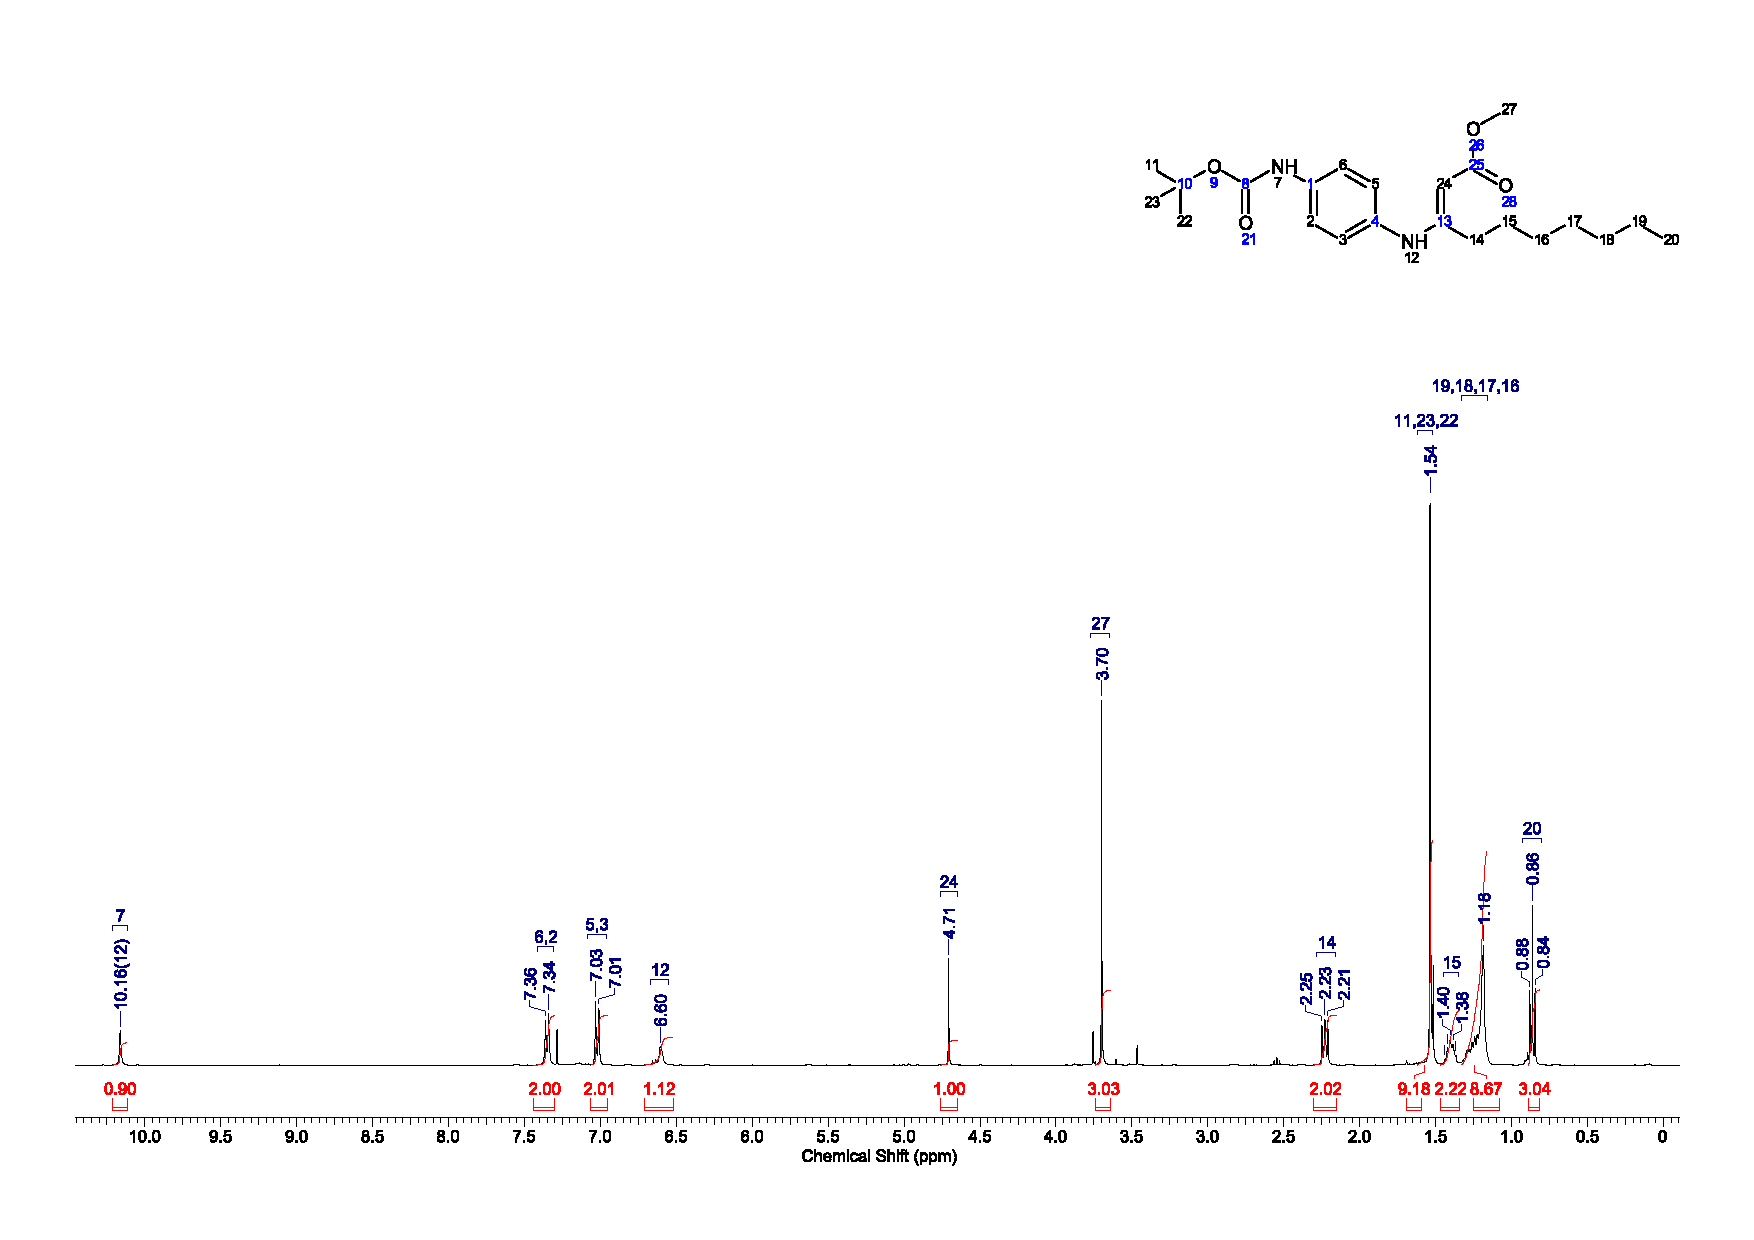
\includegraphics[ width=1.0\textwidth,height=0.43\textheight,keepaspectratio]{Bocenaman_H.pdf}
		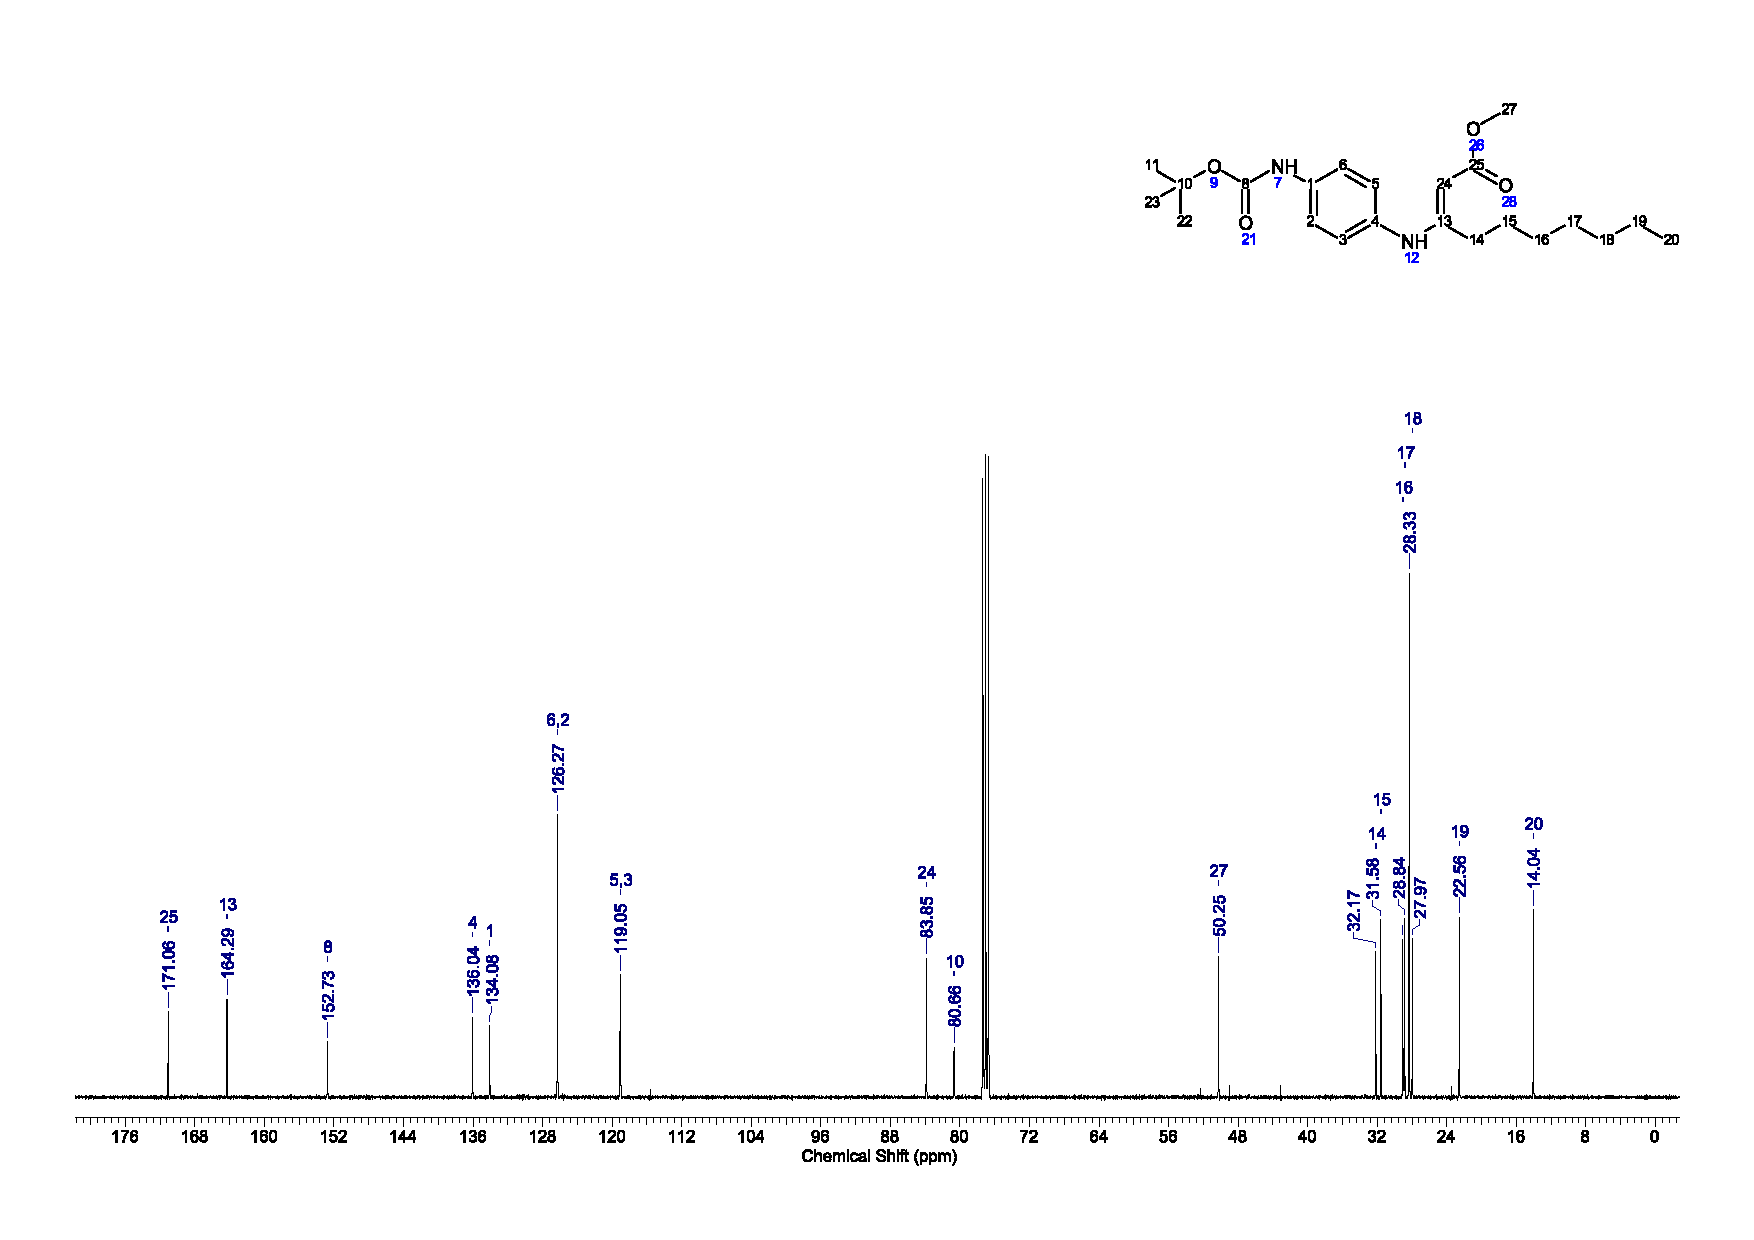
\includegraphics[ width=1.0\textwidth,height=0.43\textheight,keepaspectratio]{Bocenaman_C.pdf}
	%\caption{\compound{cmpd:Bocenaman}}
\end{figure}

\subsection{6-Amino-2-heptylquinolin-4-ol \compound{cmpd:amHHQ}}

\begin{figure}[H]
	\centering
		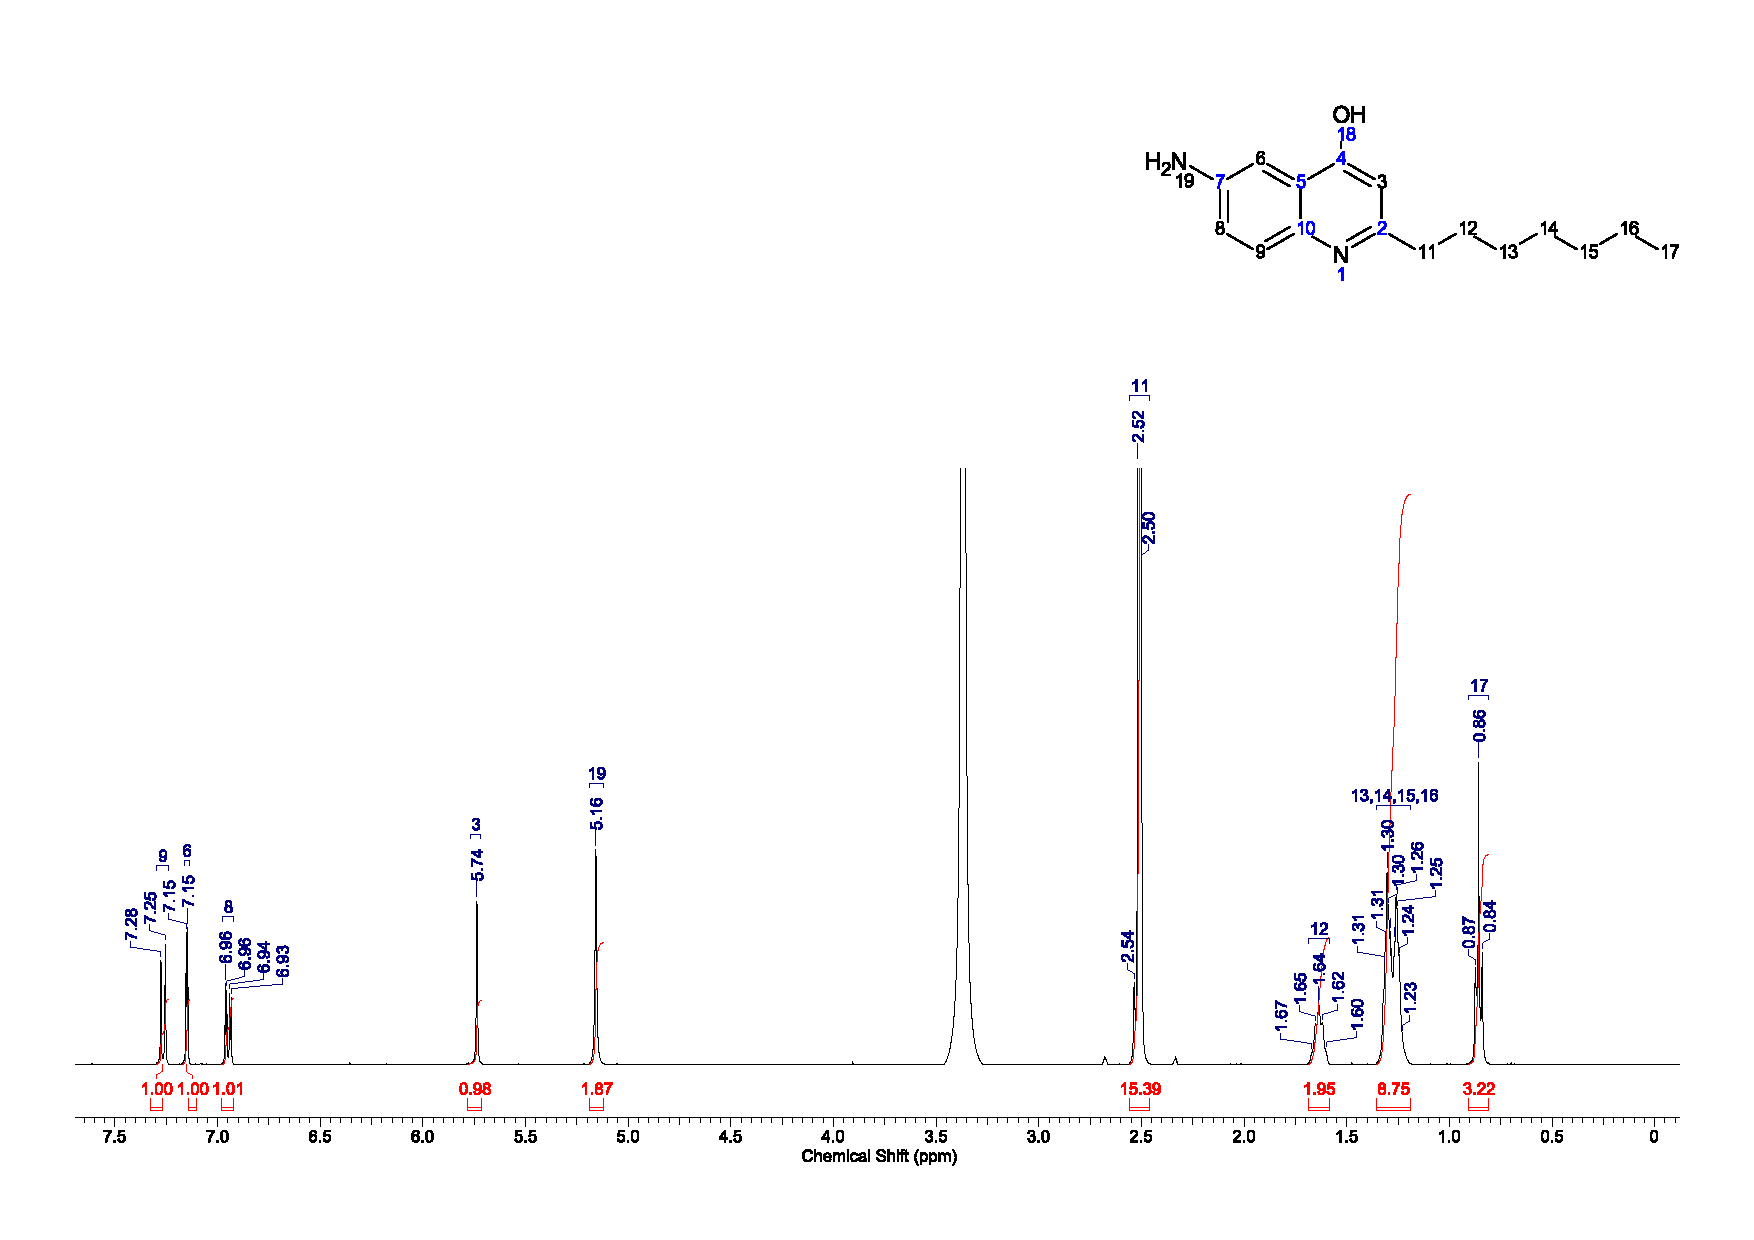
\includegraphics[ width=1.0\textwidth,height=0.43\textheight,keepaspectratio]{amHHQ_H.pdf}
		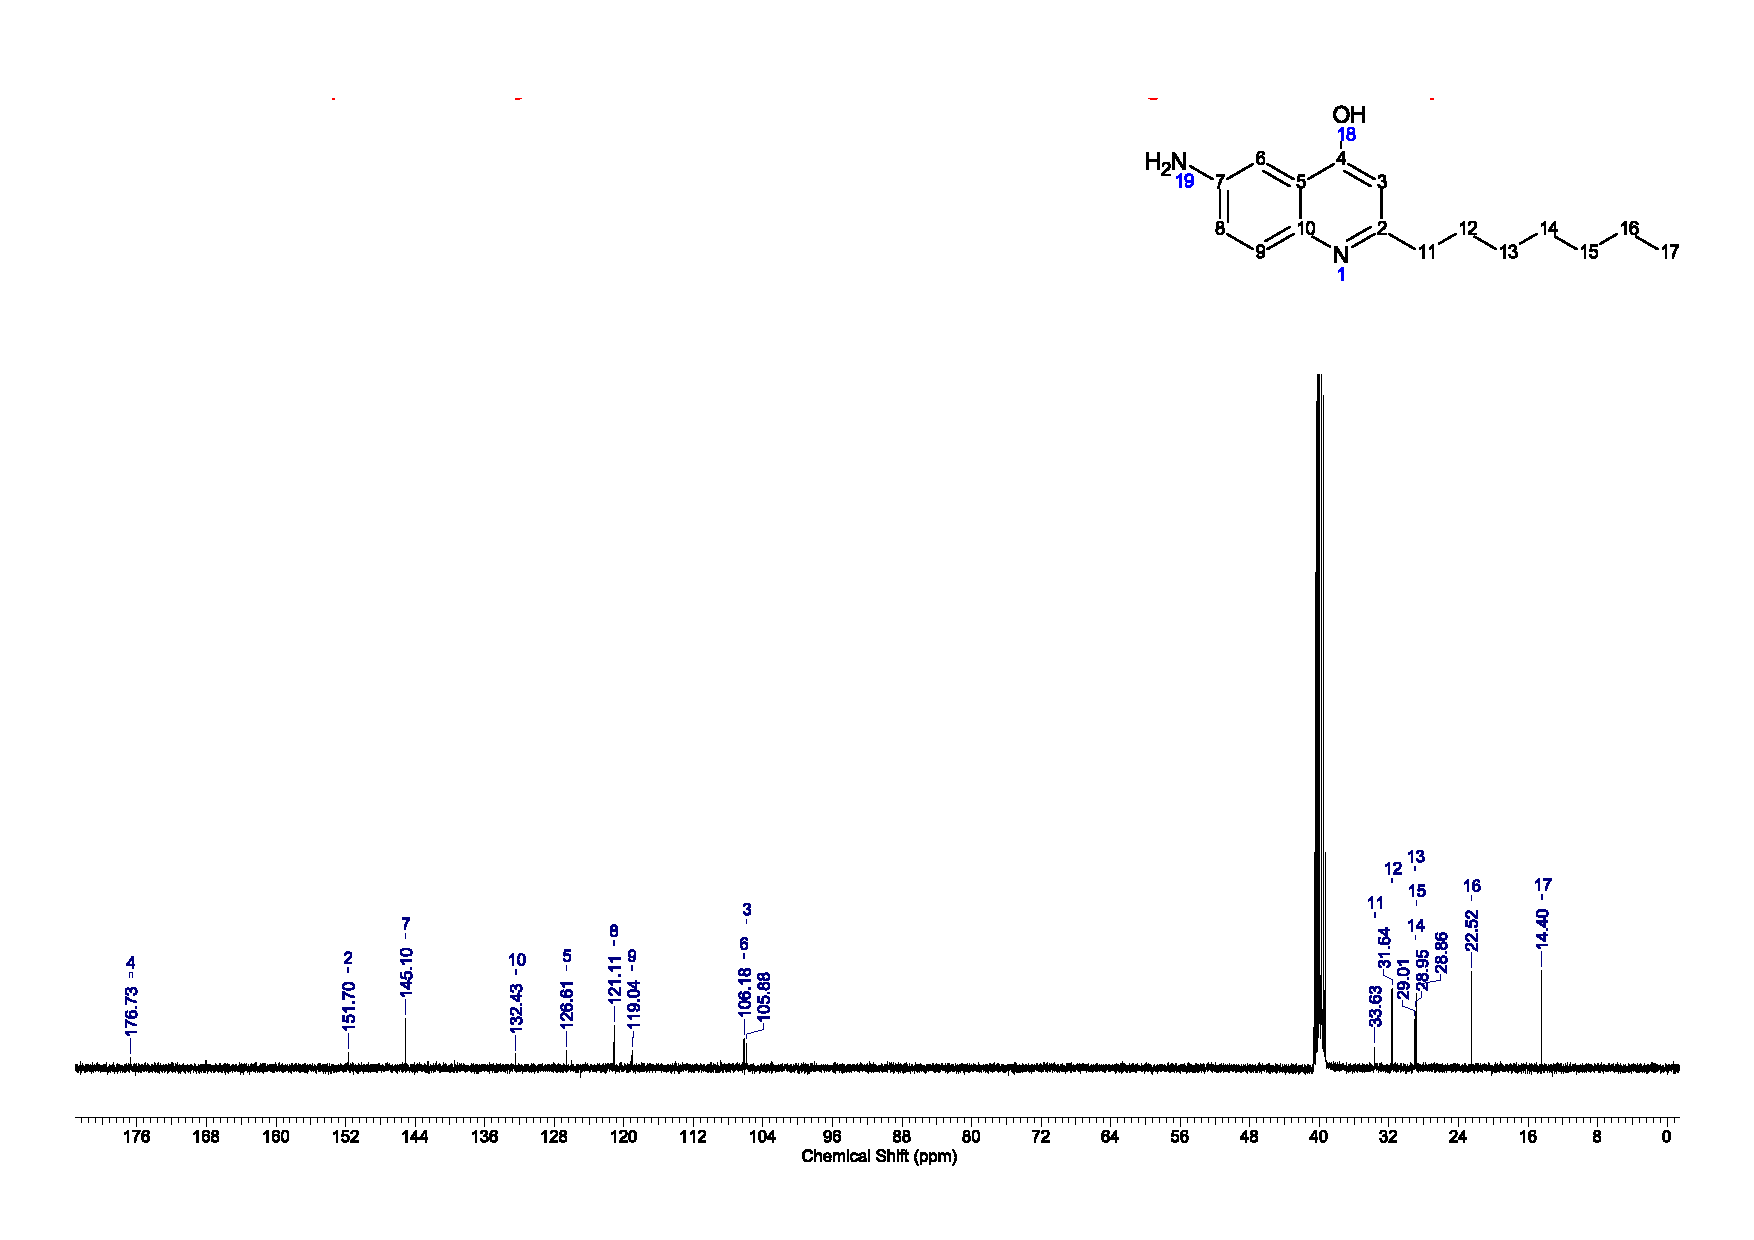
\includegraphics[ width=1.0\textwidth,height=0.43\textheight,keepaspectratio]{amHHQ_C.pdf}
	%\caption{\compound{cmpd:amHHQ}}
\end{figure}

\subsection{2-Oxononyl 2-amino-5-nitrobenzoate \compound{cmpd:5naae}}

\begin{figure}[H]
	\centering
		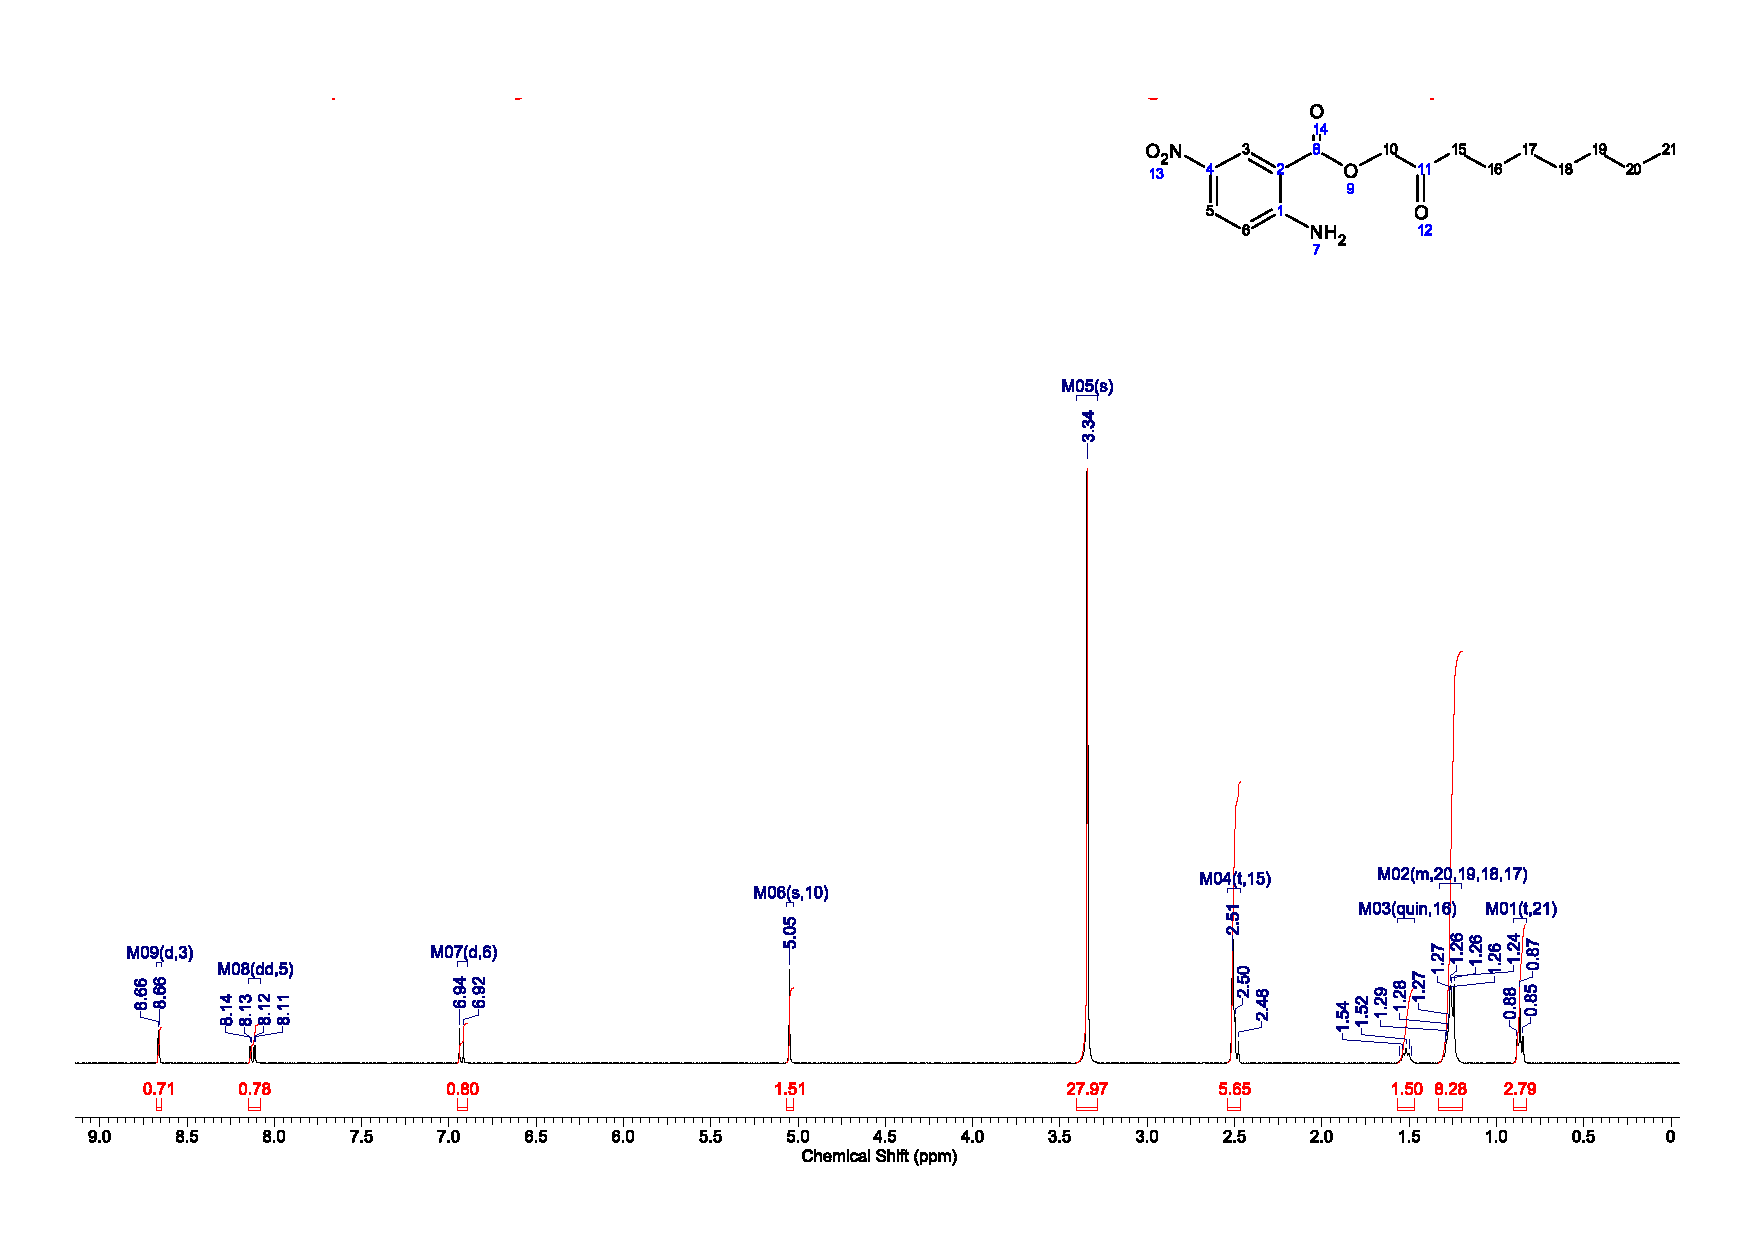
\includegraphics[ width=1.0\textwidth,height=0.43\textheight,keepaspectratio]{5Naae_H.pdf}
		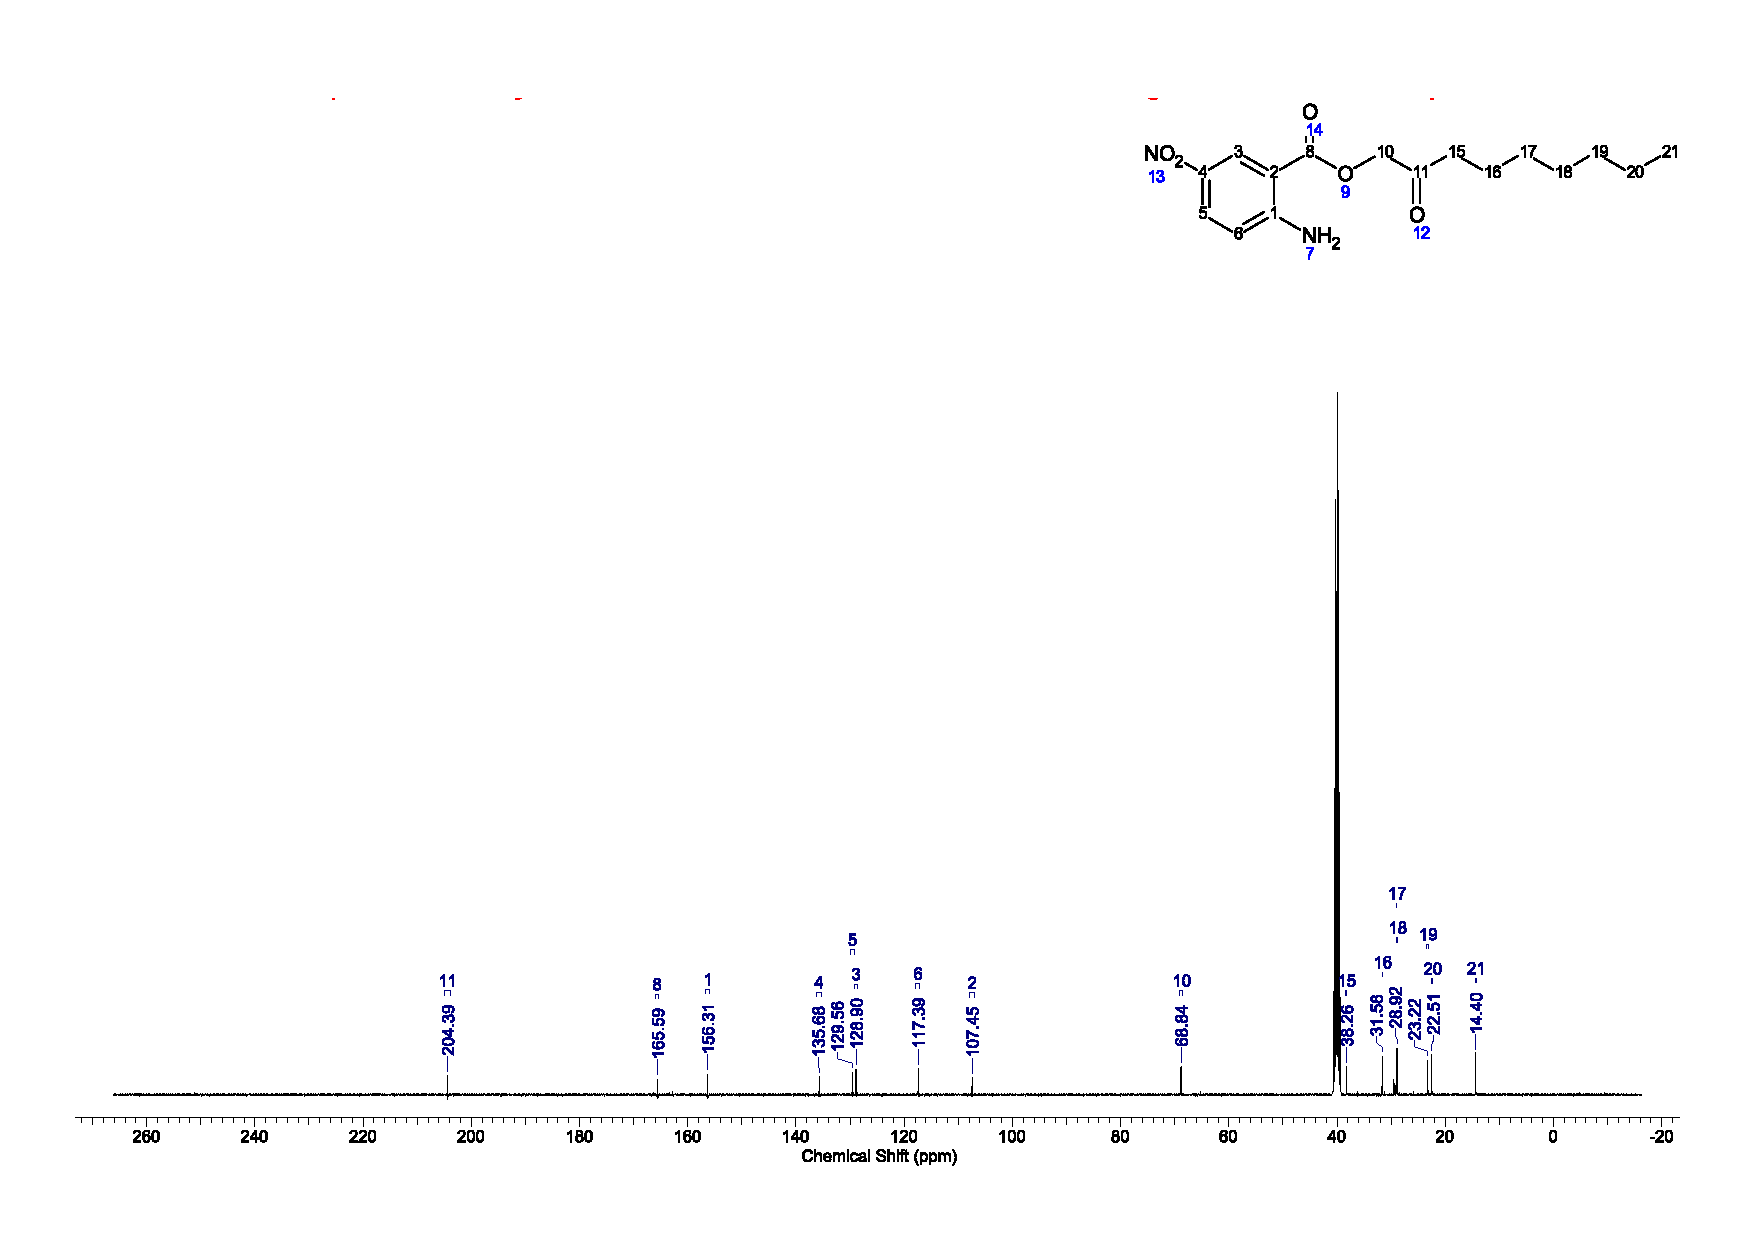
\includegraphics[ width=1.0\textwidth,height=0.43\textheight,keepaspectratio]{5Naae_C.pdf}
	%\caption{\compound{cmpd:5Naae}}
\end{figure}

\subsection{6-Nitro-2-heptyl-3-hydroxyquinolin-4(1\textit{H})-one \compound{cmpd:NPQS}}

\begin{figure}[H]
	\centering
		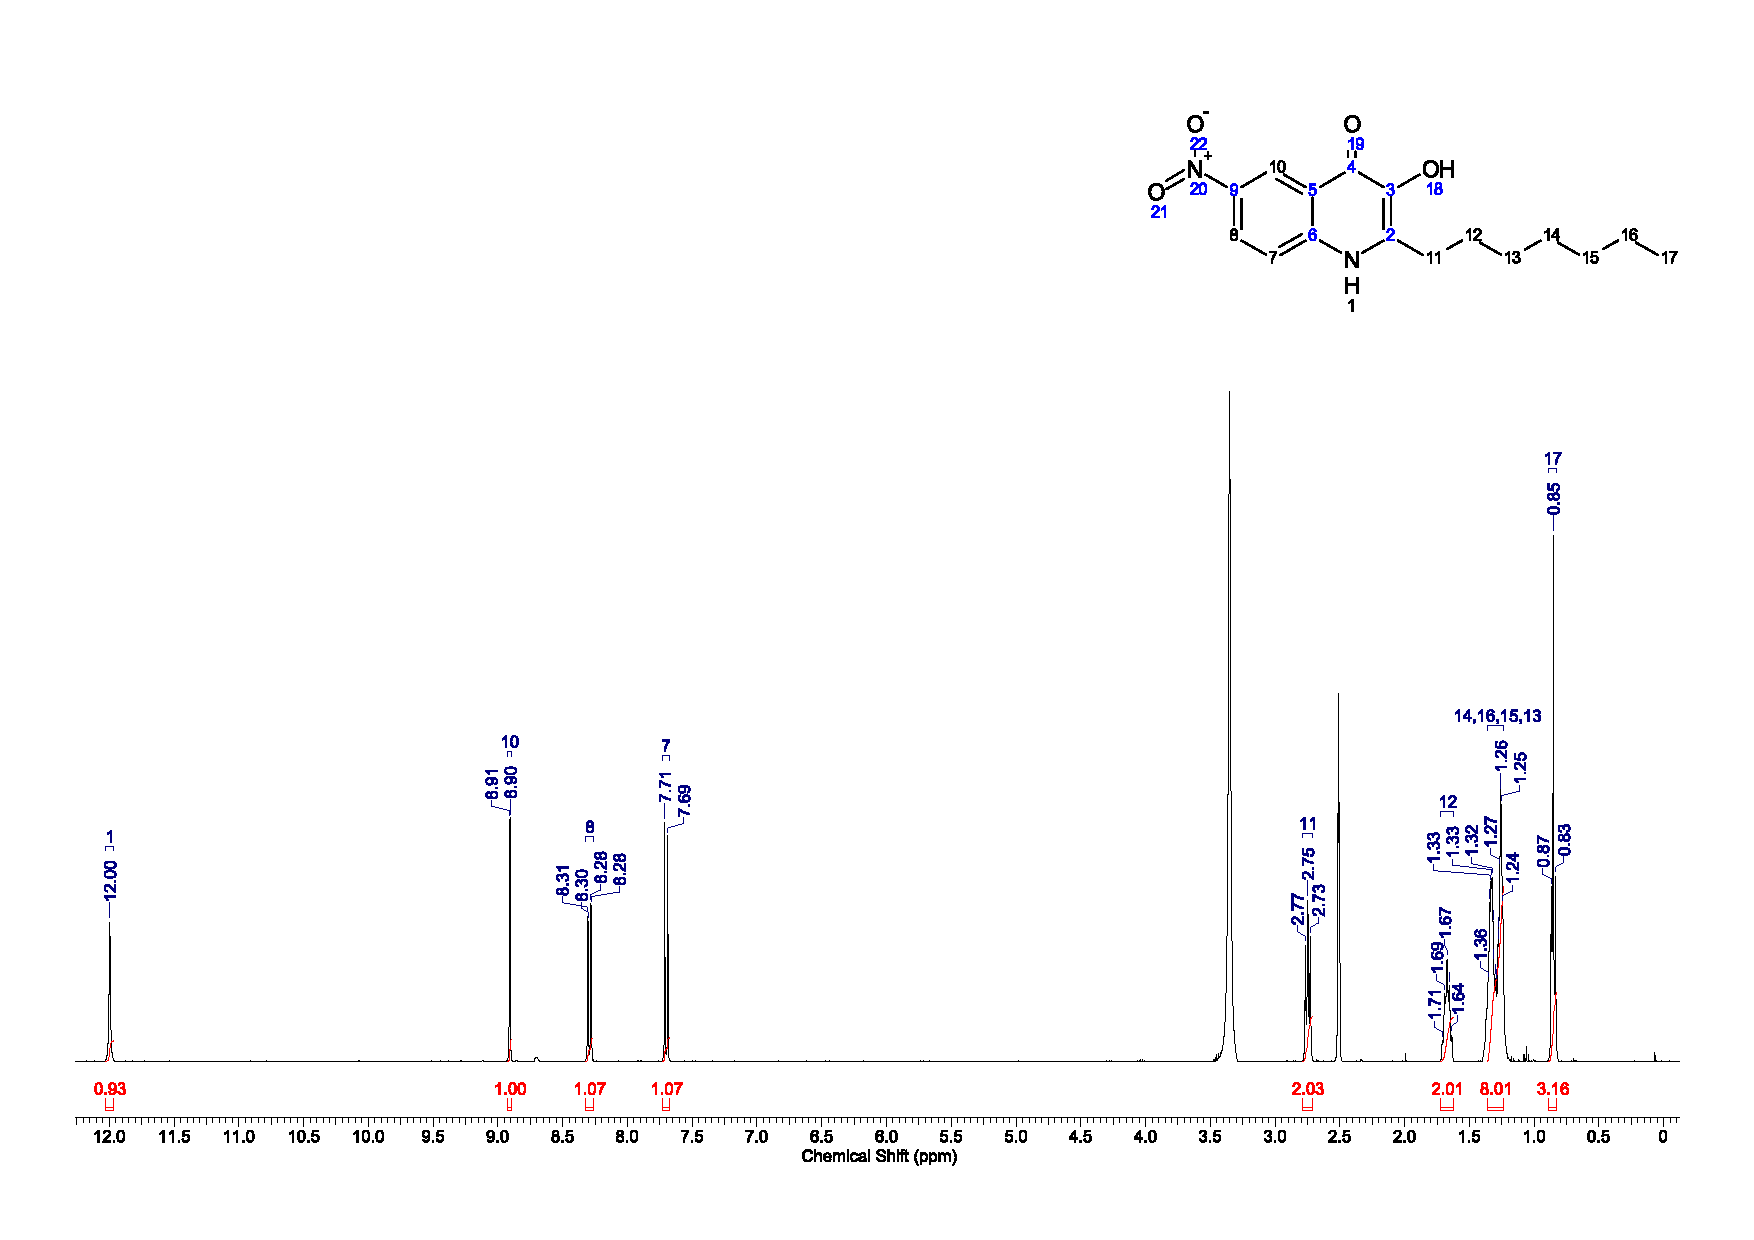
\includegraphics[ width=1.0\textwidth,height=0.43\textheight,keepaspectratio]{NPQS_H.pdf}
		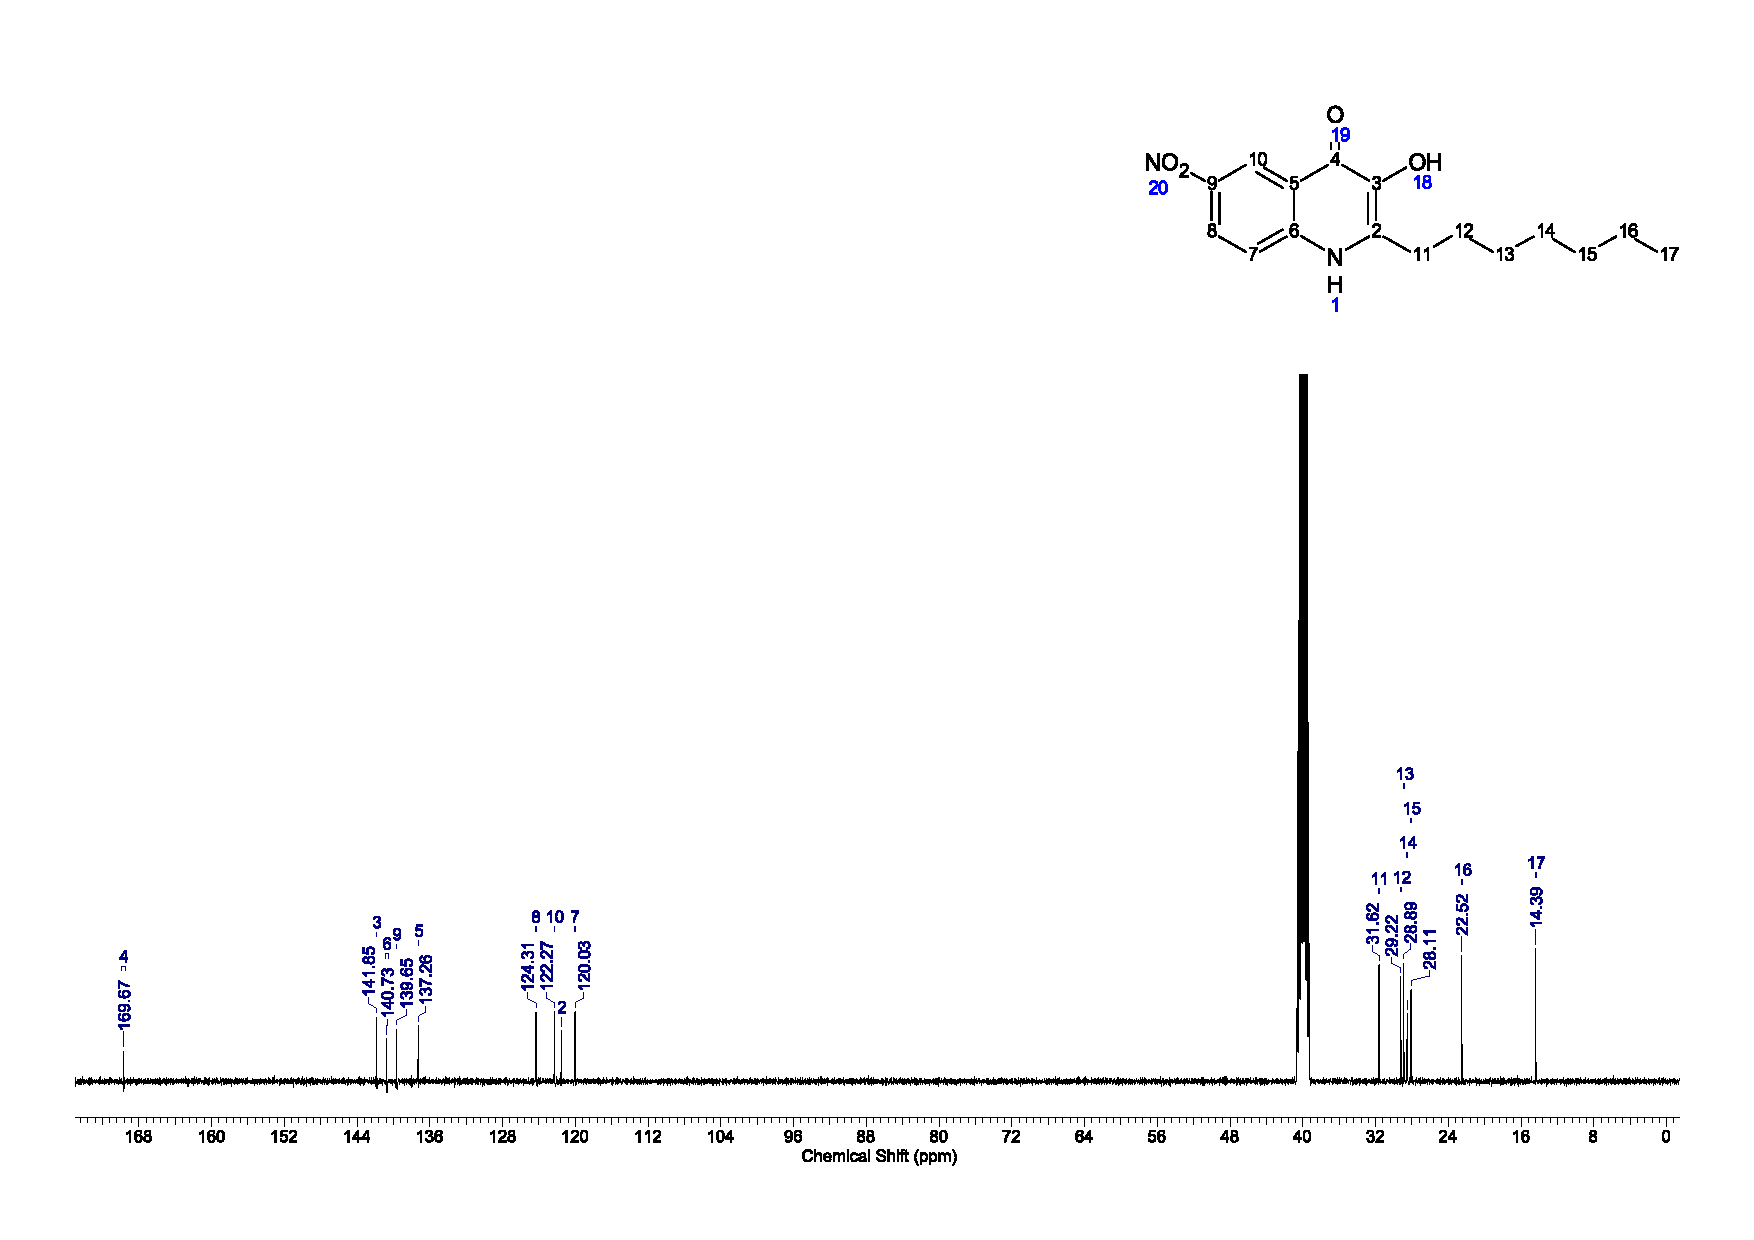
\includegraphics[ width=1.0\textwidth,height=0.43\textheight,keepaspectratio]{NPQS_C.pdf}
	%\caption{\compound{cmpd:NPQS}}
\end{figure}

\subsection{6-Amino-2-heptyl-3-hydroxyquinolin-4(1\textit{H})-one \compound{cmpd:amPQS}}

\begin{figure}[H]
	\centering
		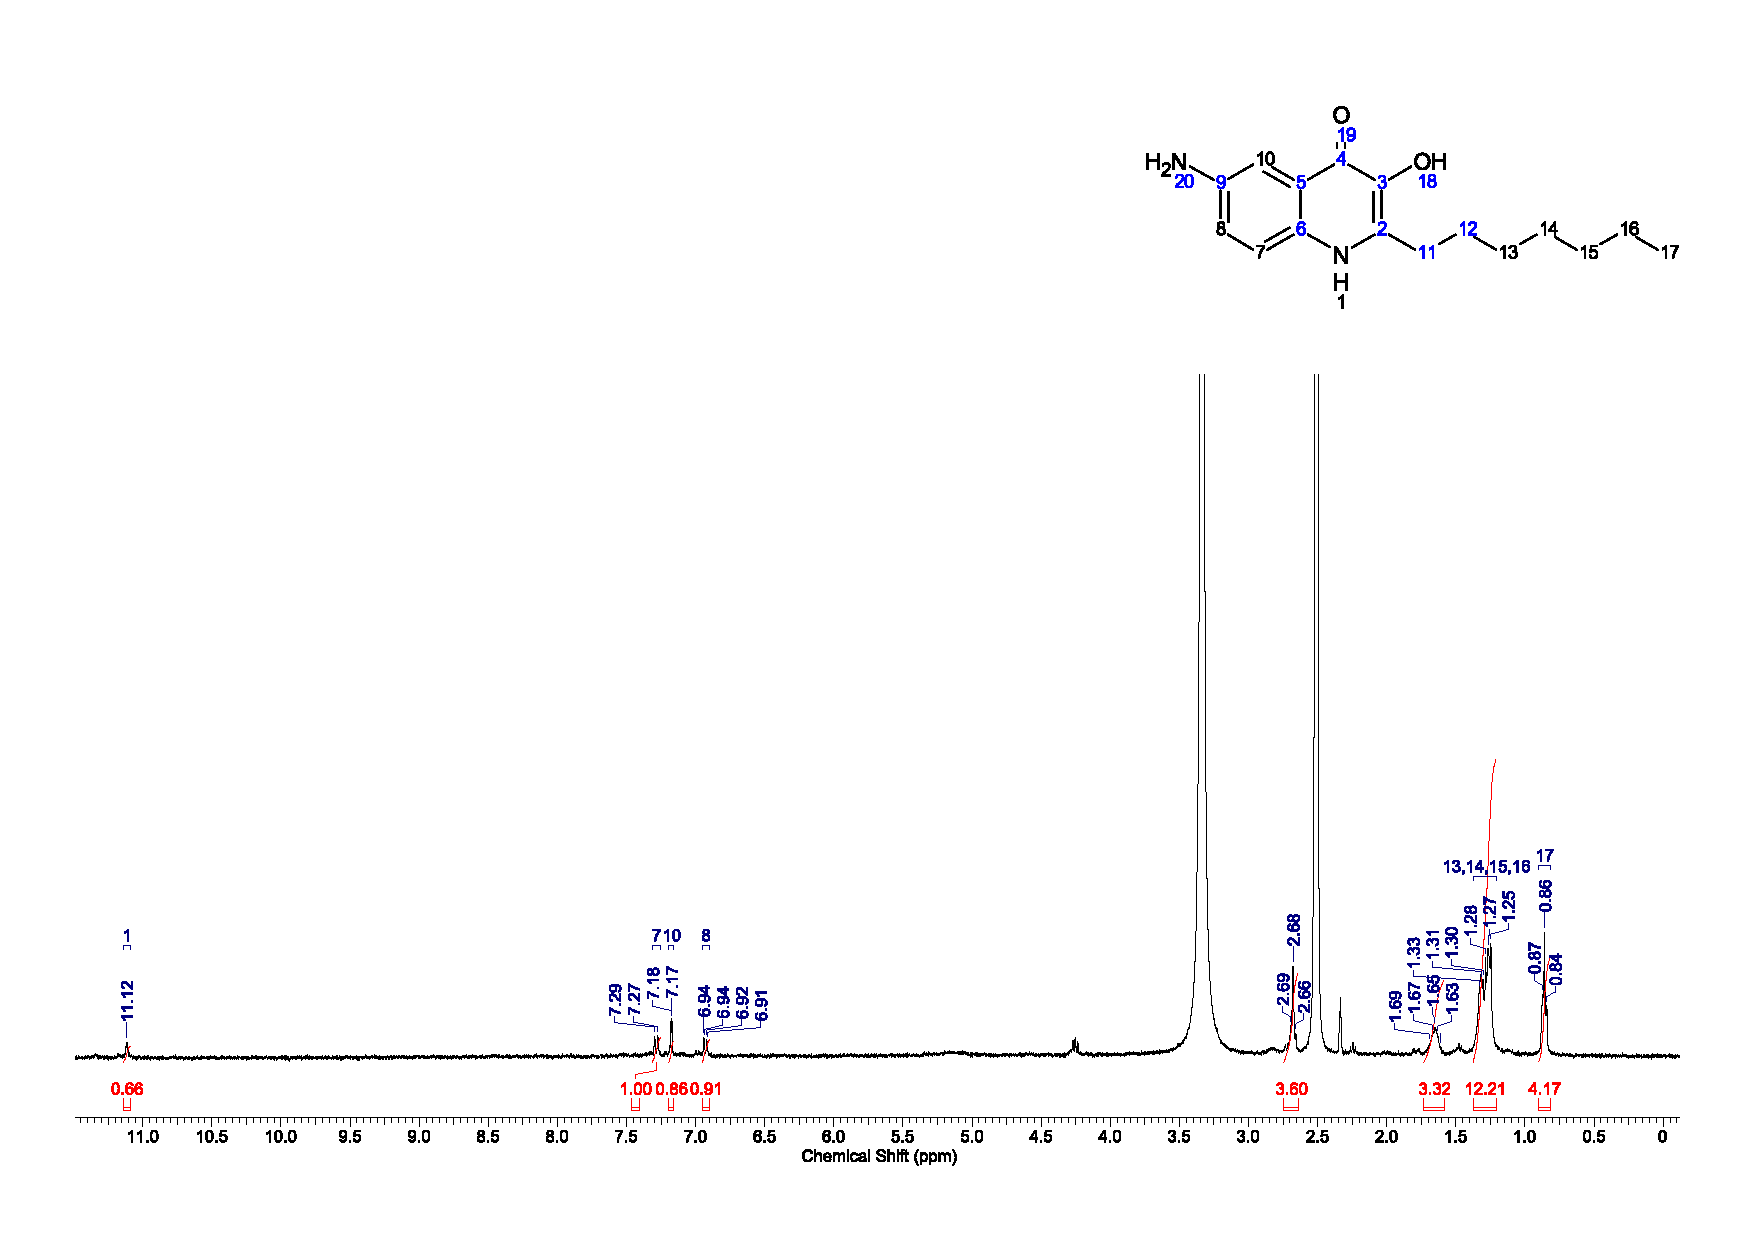
\includegraphics[ width=1.0\textwidth,height=0.43\textheight,keepaspectratio]{amPQS_H.pdf}
		%\includegraphics[ width=1.0\textwidth,height=0.43\textheight,keepaspectratio]{amPQS_C.pdf}
	%\caption{\compound{cmpd:amPQS}}
\end{figure}

\subsection{6-Azido-2-heptyl-3-hydroxyquinolin-4(1\textit{H})-one \compound{cmpd:azPQS}}

\begin{figure}[H]
	\centering
		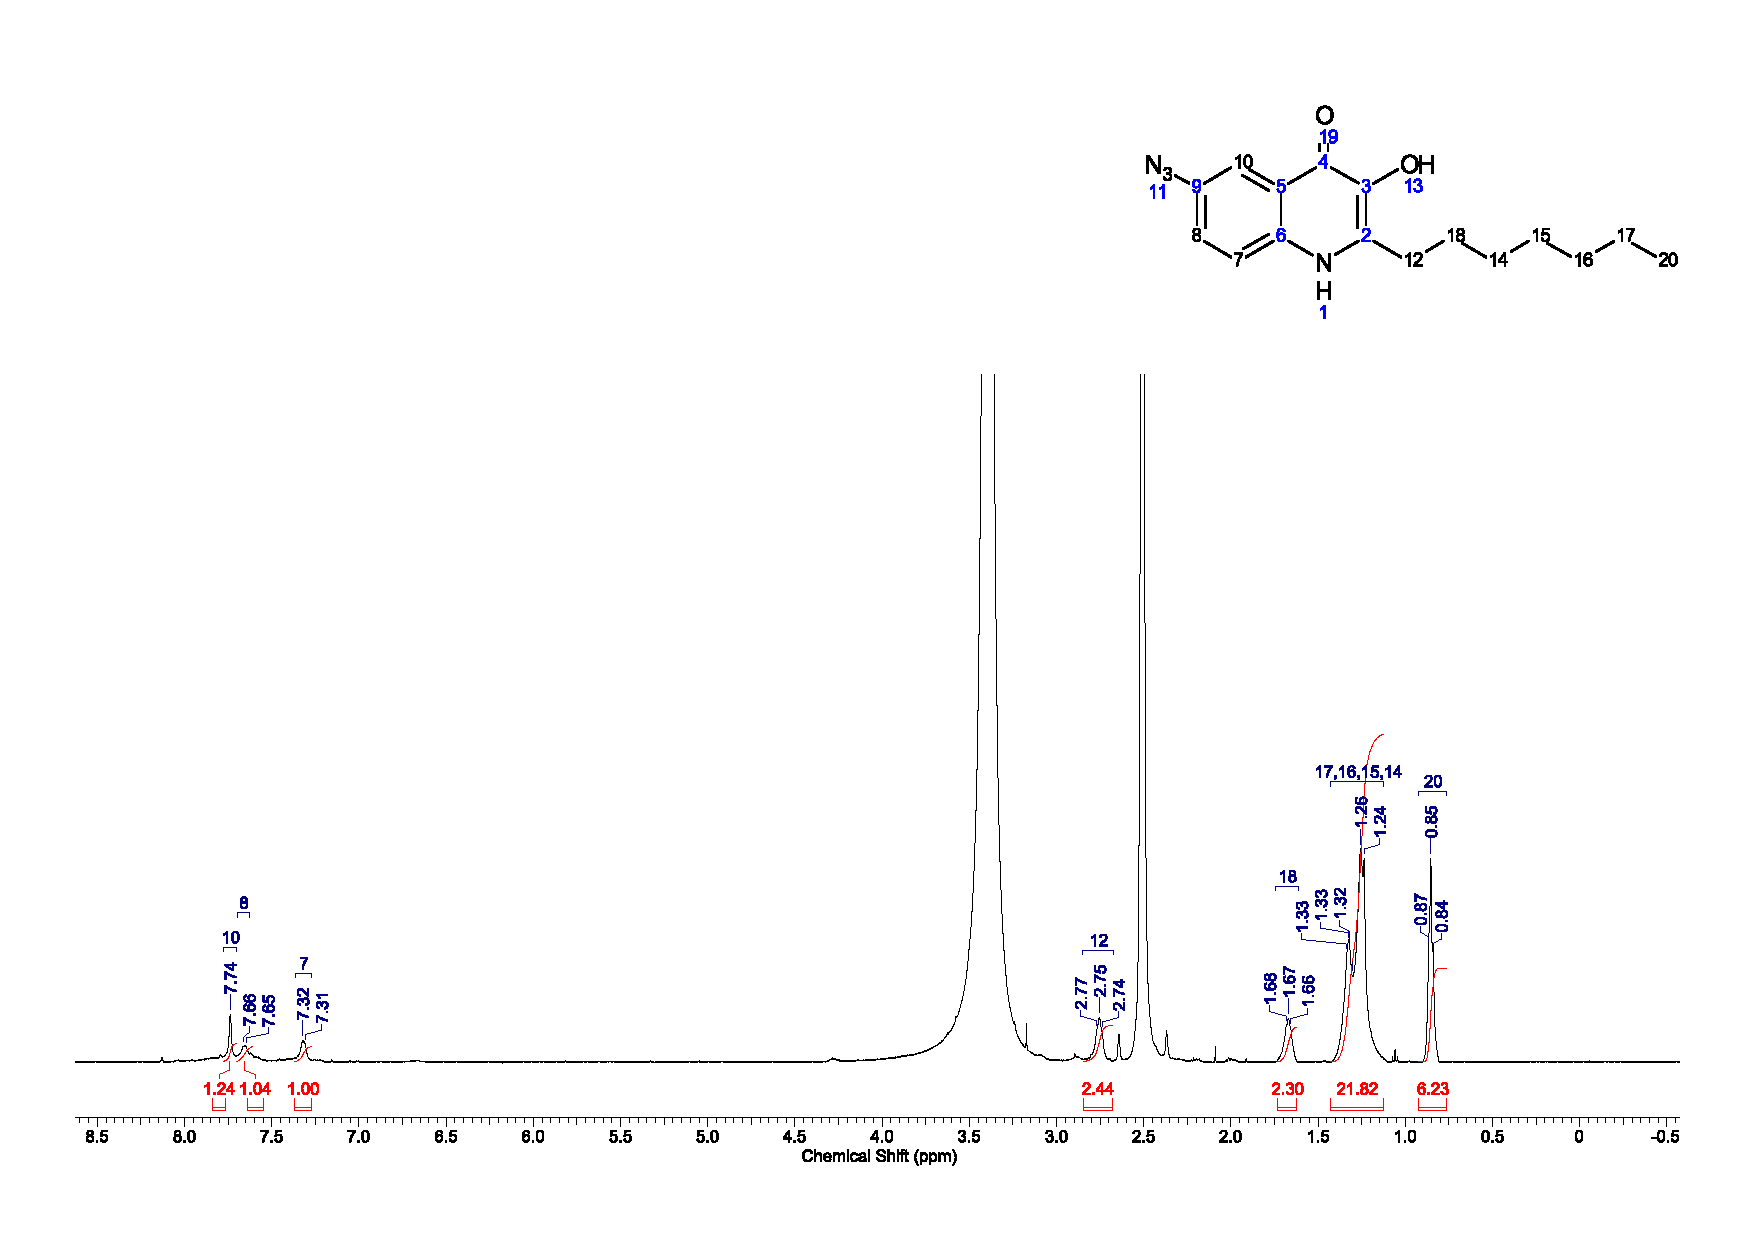
\includegraphics[ width=1.0\textwidth,height=0.43\textheight,keepaspectratio]{azPQS_H.pdf}
	%\caption{\compound{cmpd:azPQS}}
\end{figure}

\subsection{(\textit{S})-4-Bromo-\textit{N}-(2-oxotetrahydrofuran-3-yl)butanamide \compound{cmpd:HL4Br}}

\begin{figure}[H]
	\centering
		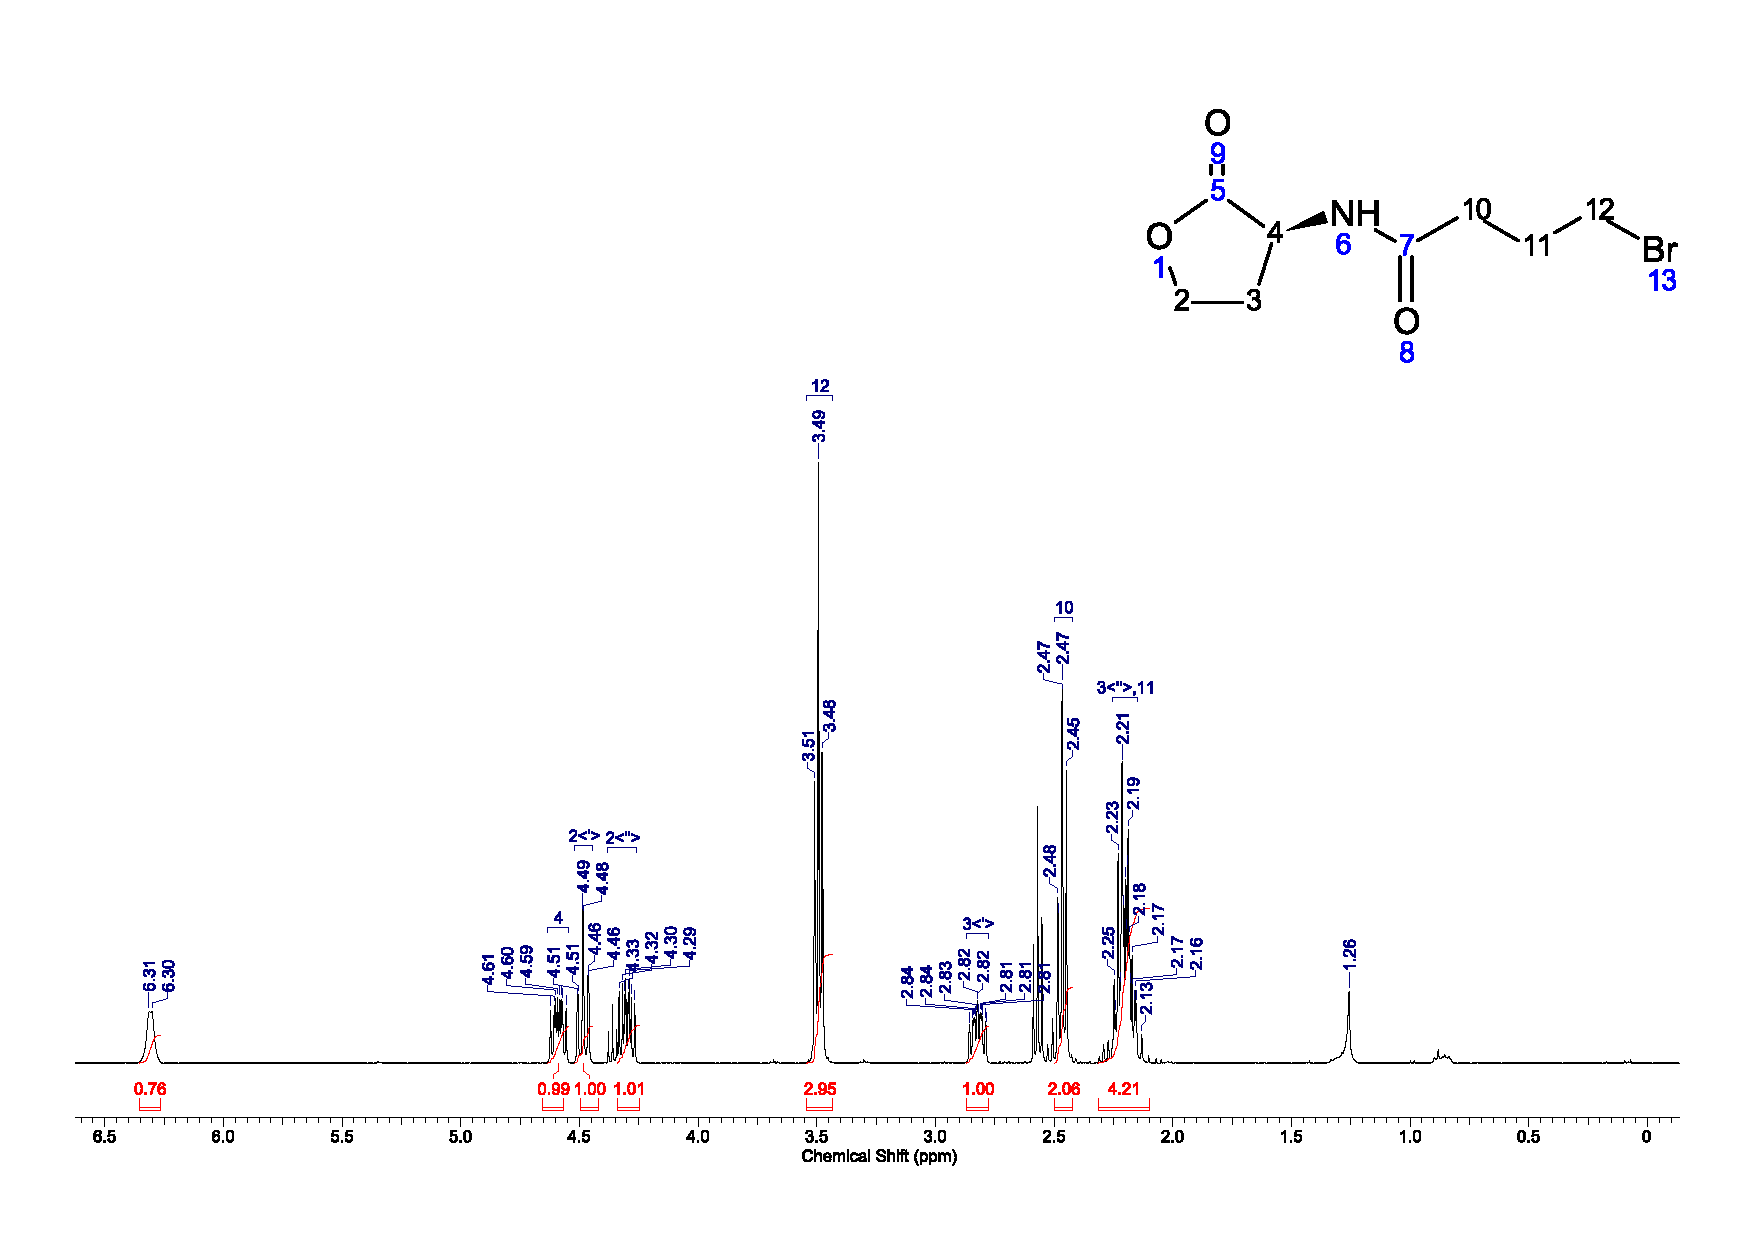
\includegraphics[ width=1.0\textwidth,height=0.43\textheight,keepaspectratio]{HL4Br_H.pdf}
		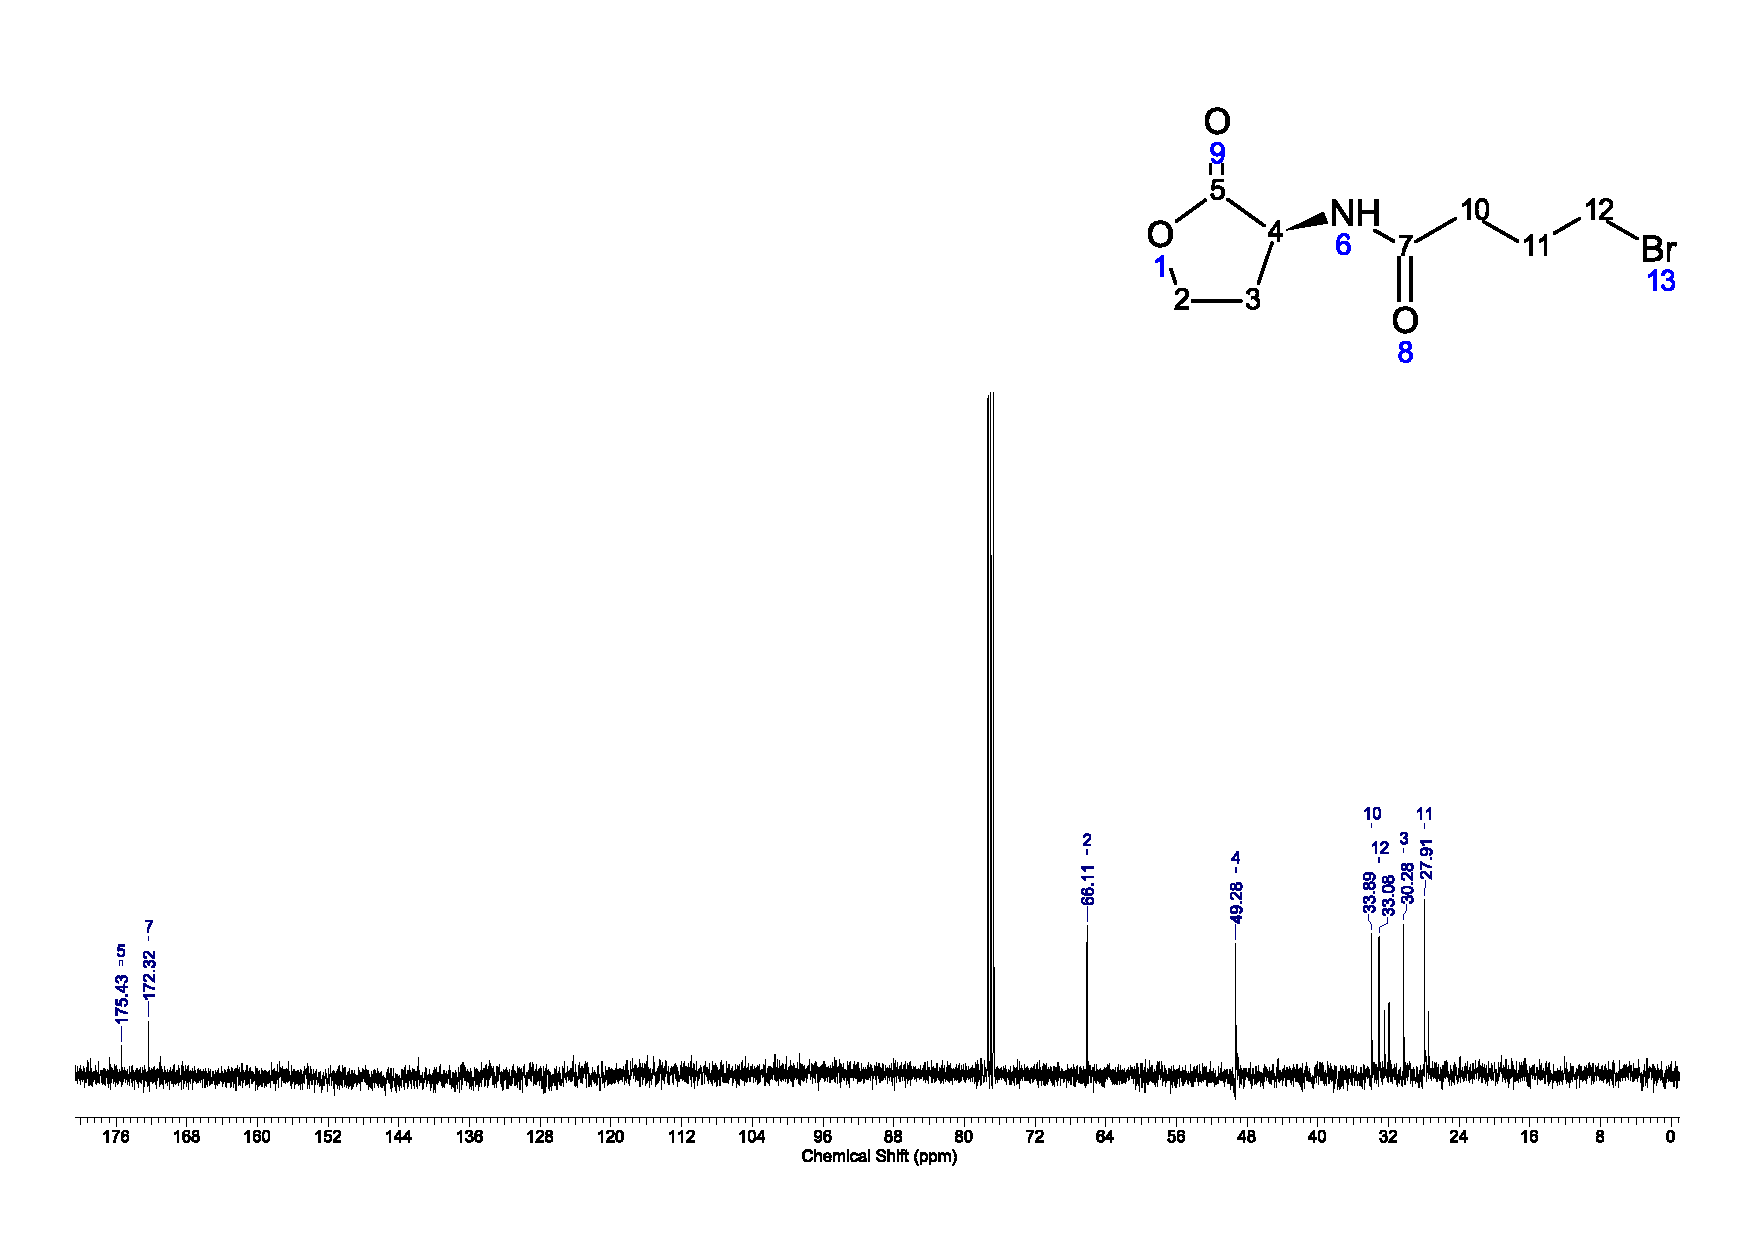
\includegraphics[ width=1.0\textwidth,height=0.43\textheight,keepaspectratio]{HL4Br_C.pdf}
	%\caption{\compound{cmpd:HL4Br}}
\end{figure}

\subsection{(\textit{S})-6-Bromo-\textit{N}-(2-oxotetrahydrofuran-3-yl)hexanamide \compound{cmpd:HL6Br}}

\begin{figure}[H]
	\centering
		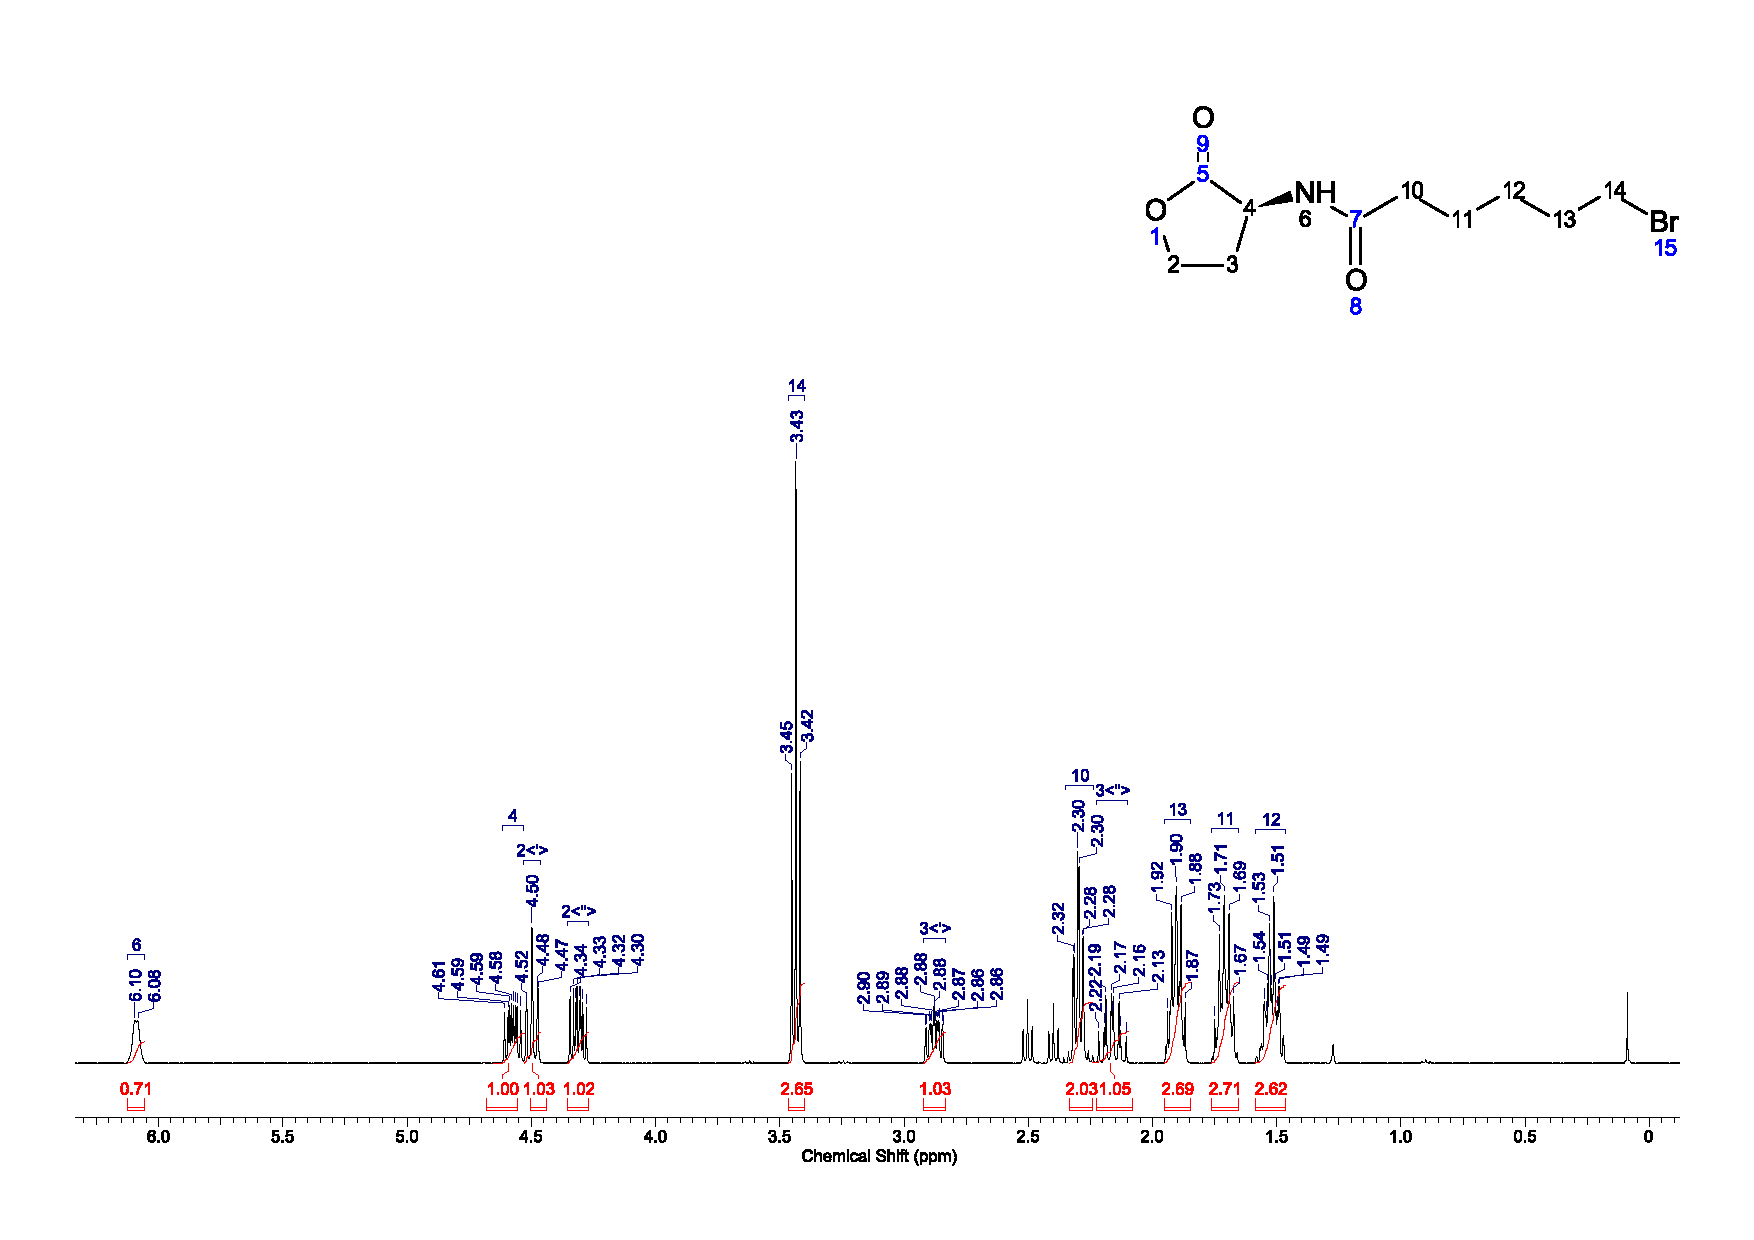
\includegraphics[ width=1.0\textwidth,height=0.43\textheight,keepaspectratio]{HL6Br_H.pdf}
		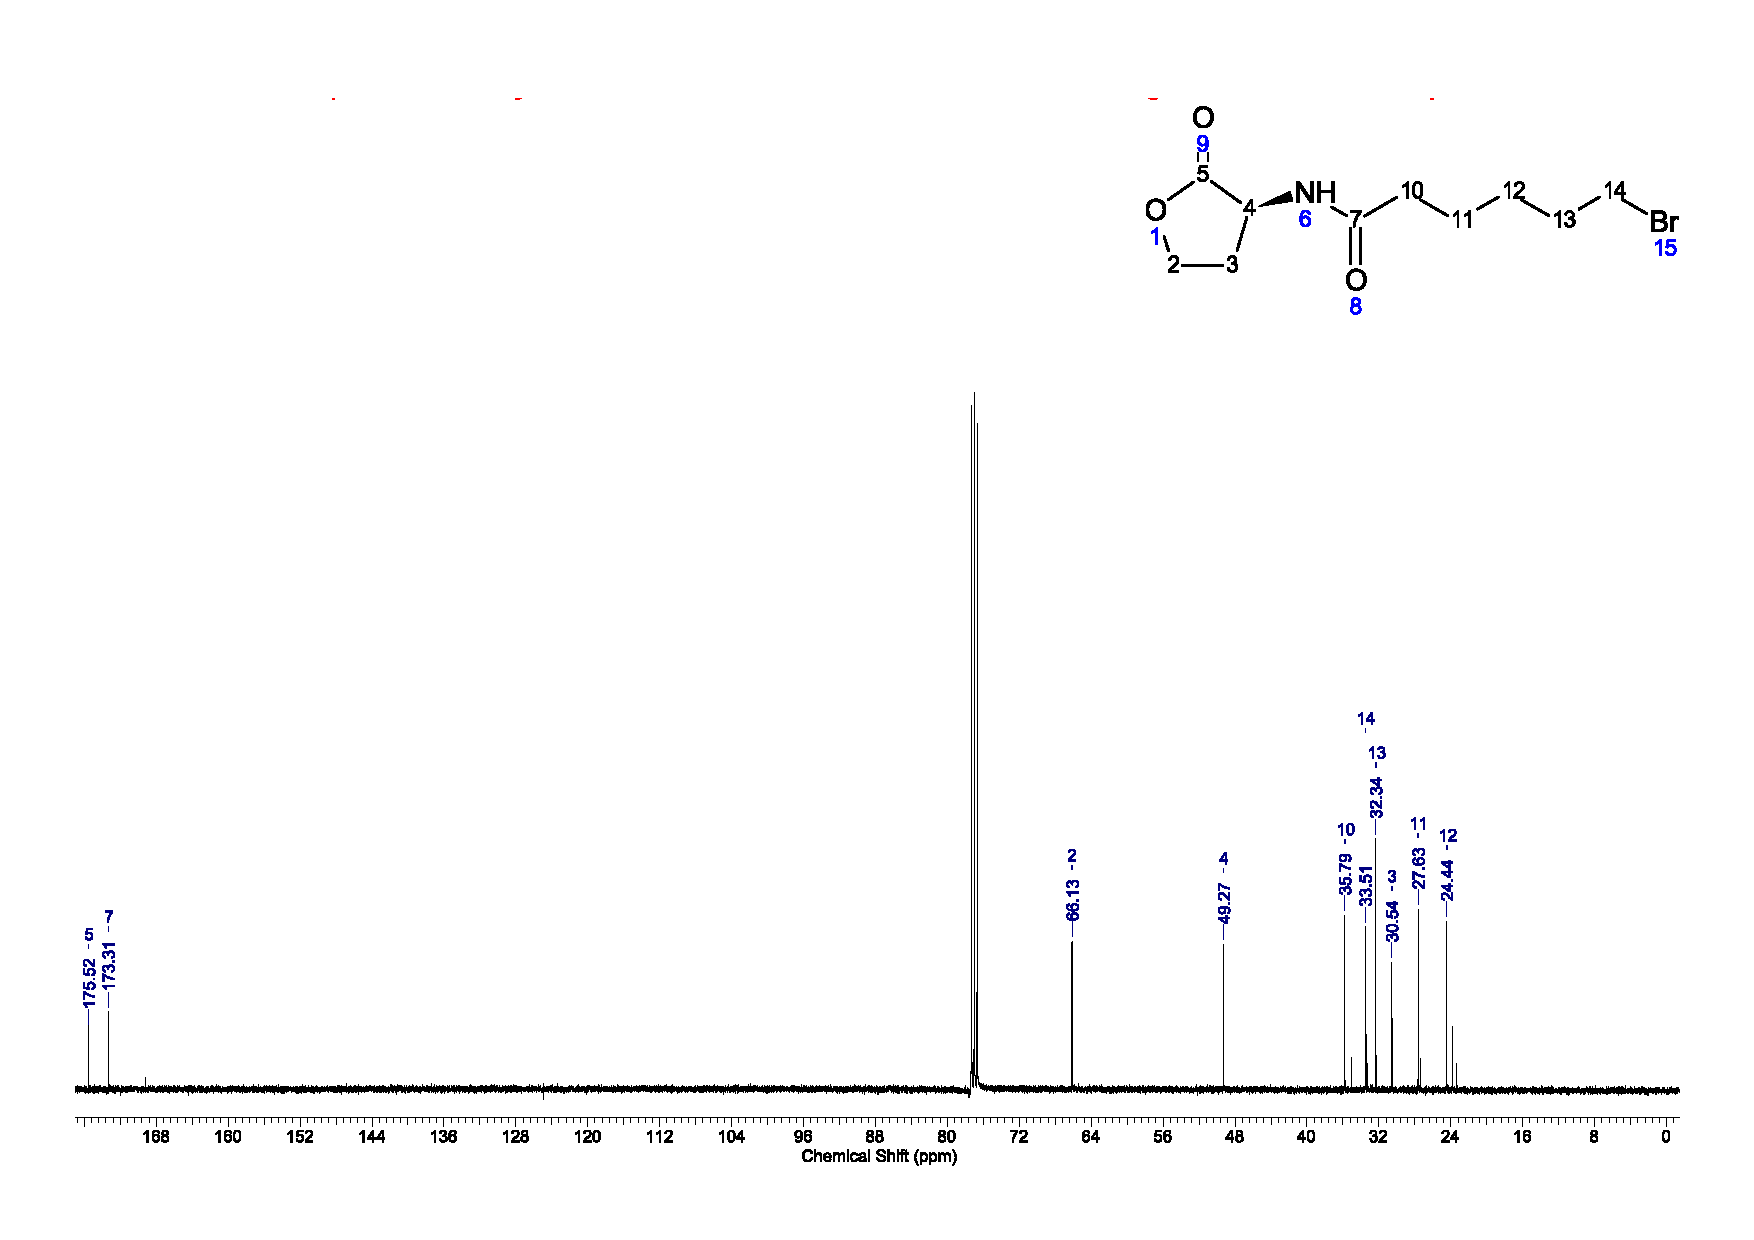
\includegraphics[ width=1.0\textwidth,height=0.43\textheight,keepaspectratio]{HL6Br_C.pdf}
	%\caption{\compound{cmpd:HL6Br}}
\end{figure}

\subsection{(\textit{S})-6-Azido-\textit{N}-(2-oxotetrahydrofuran-3-yl)hexanamide \compound{cmpd:HL6N3}}

\begin{figure}[H]
	\centering
		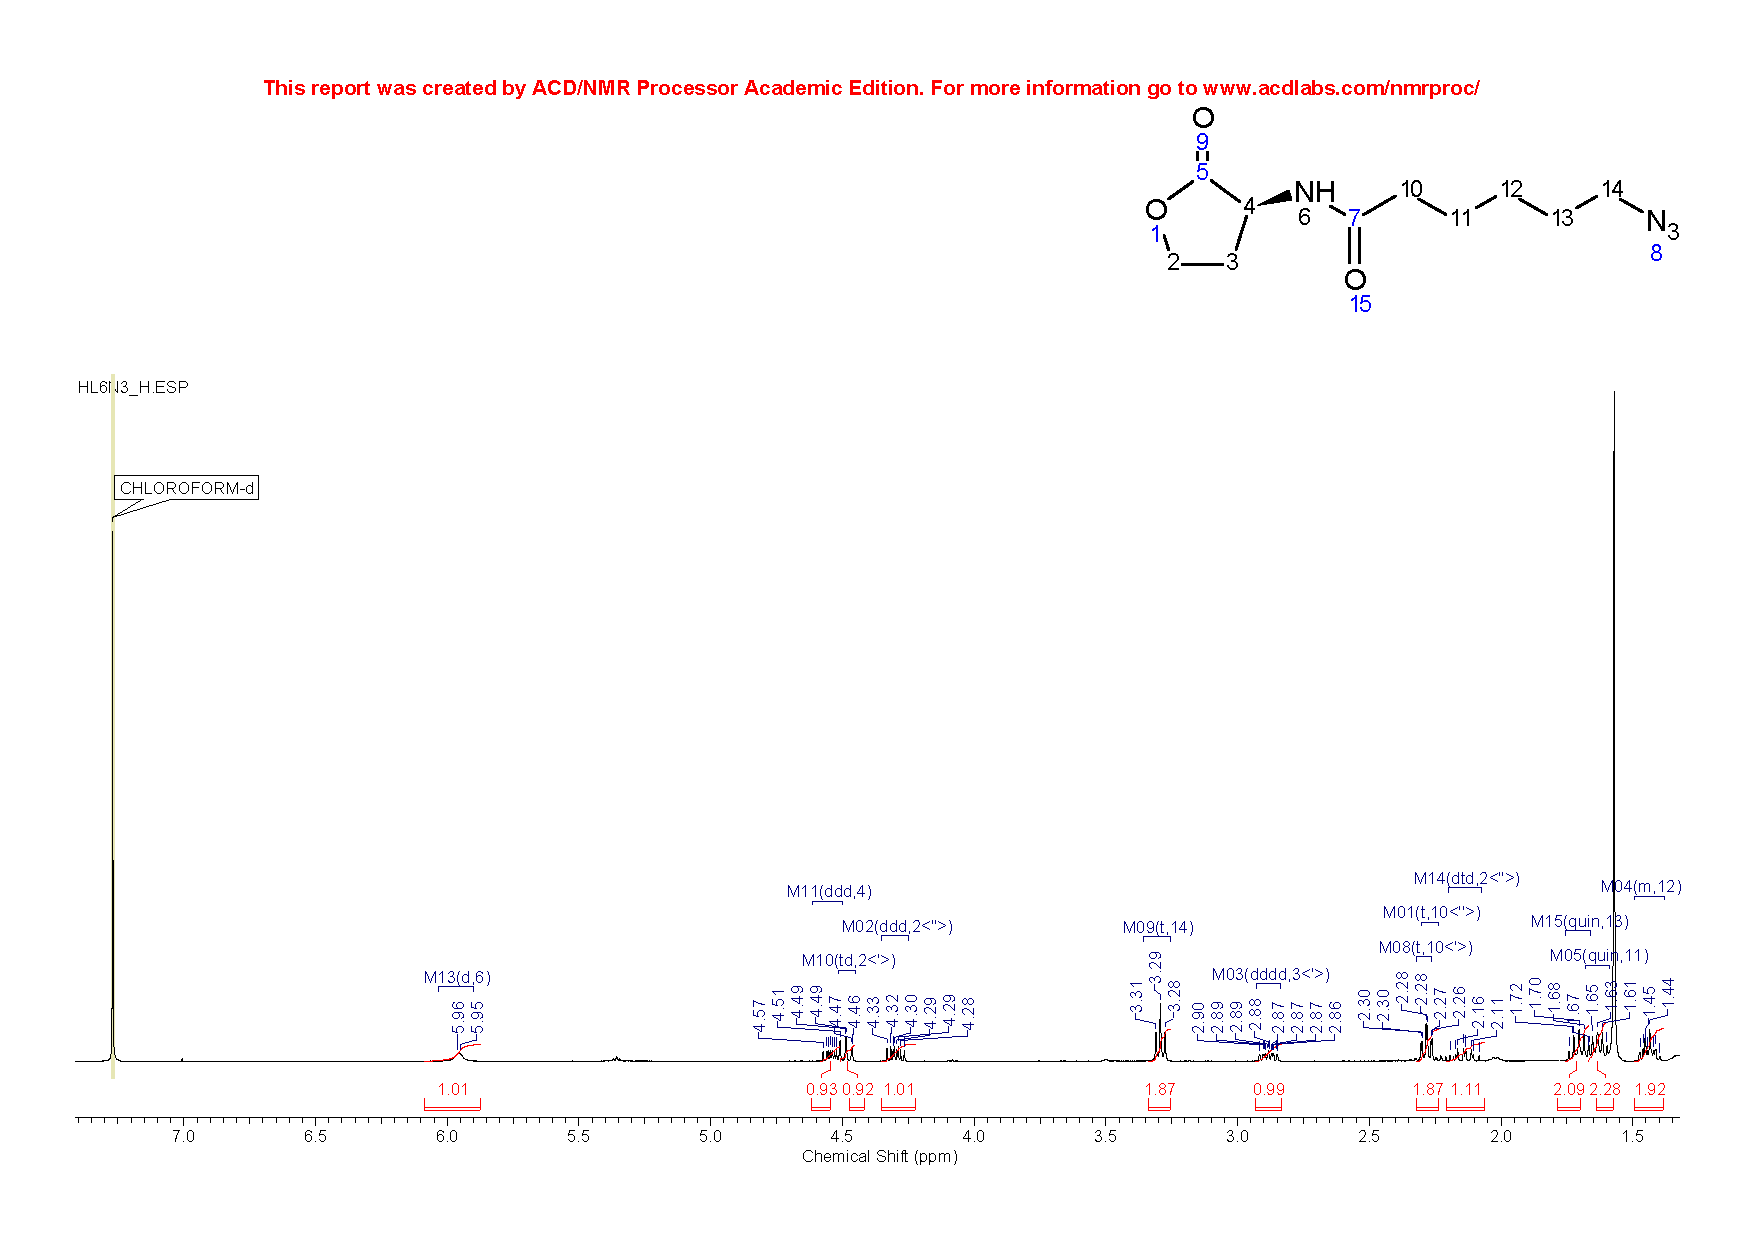
\includegraphics[ width=1.0\textwidth,height=0.43\textheight,keepaspectratio]{HL6N3_H.pdf}
		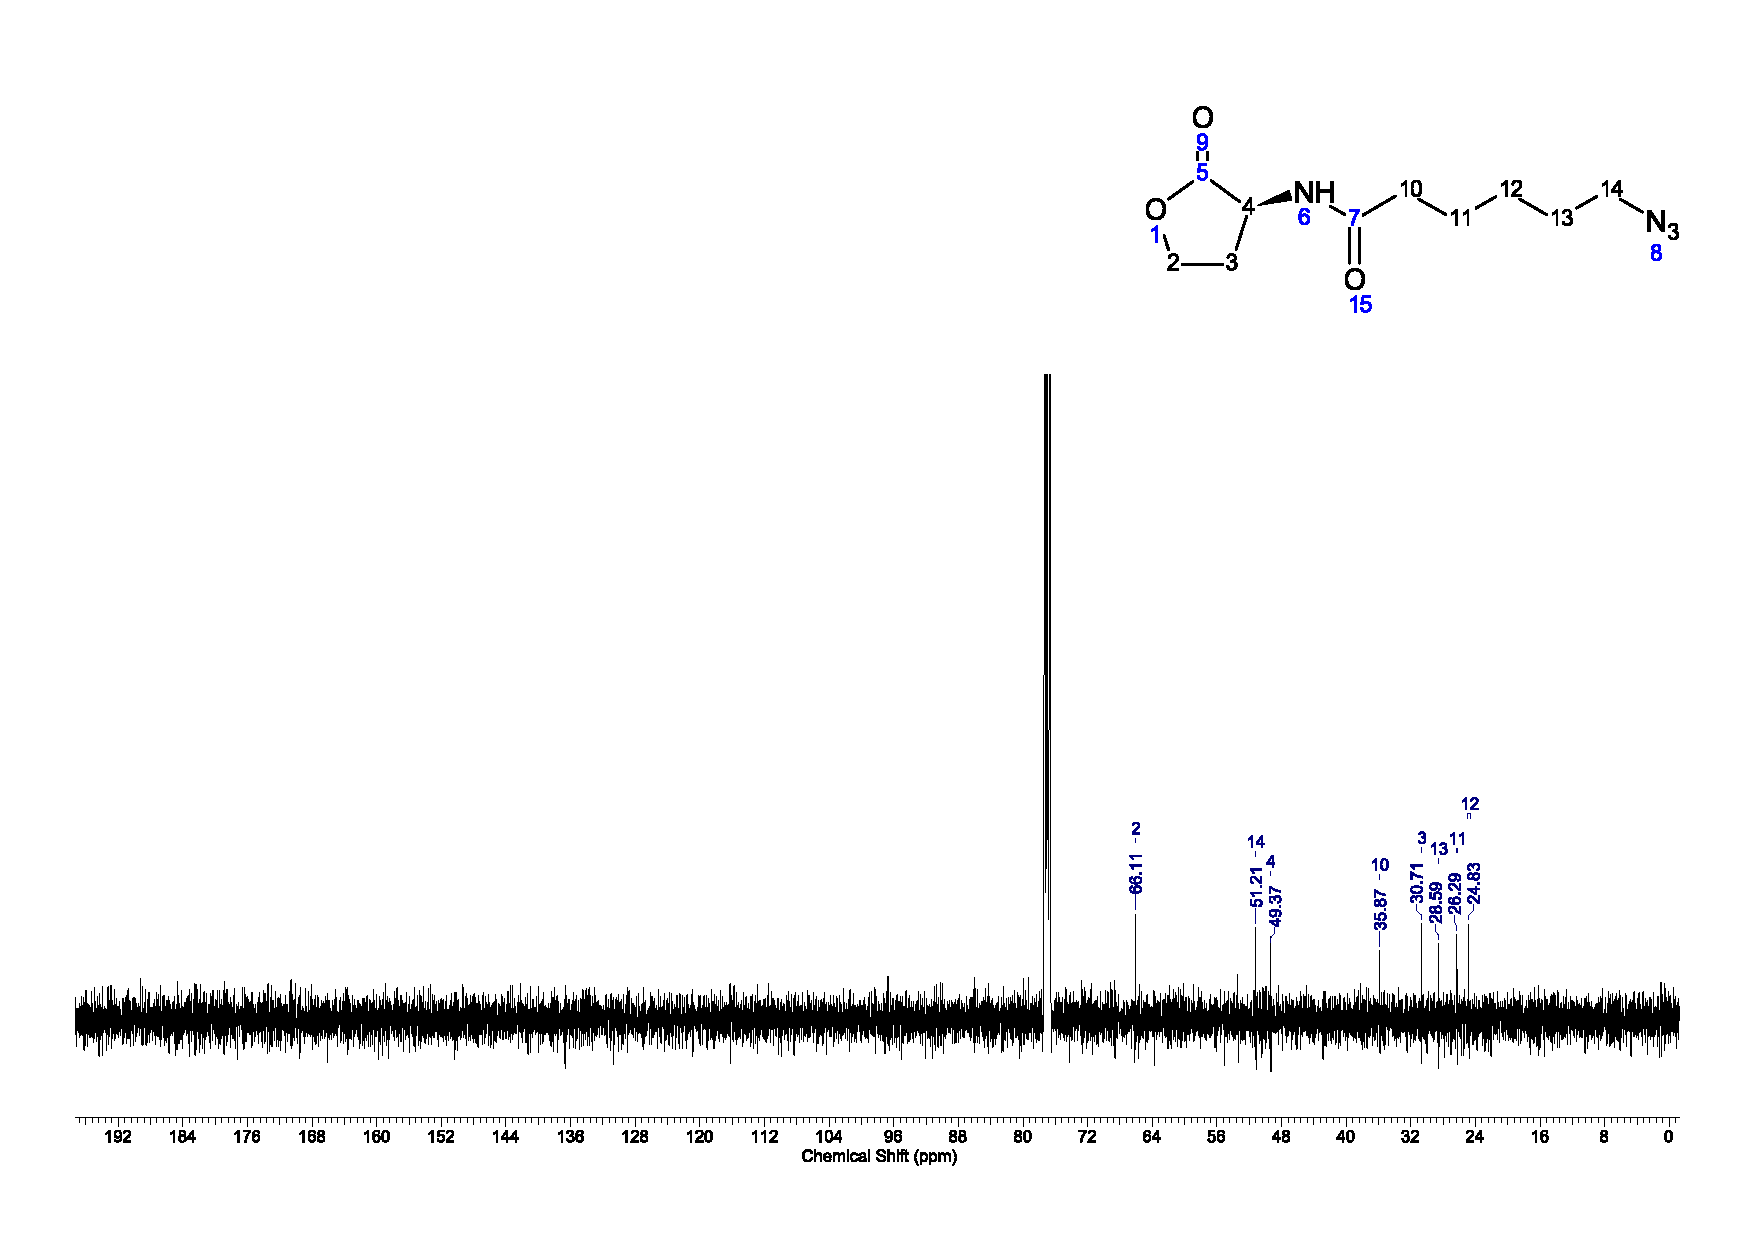
\includegraphics[ width=1.0\textwidth,height=0.43\textheight,keepaspectratio]{HL6N3_C.pdf}
	%\caption{\compound{cmpd:HL6N3}}
\end{figure}

\subsection{\textit{tert}-Butyl 4-(hex-5-yn-1-yl)piperazine-1-carboxylate \compound{cmpd:hexpipboc}}

\begin{figure}[H]
	\centering
		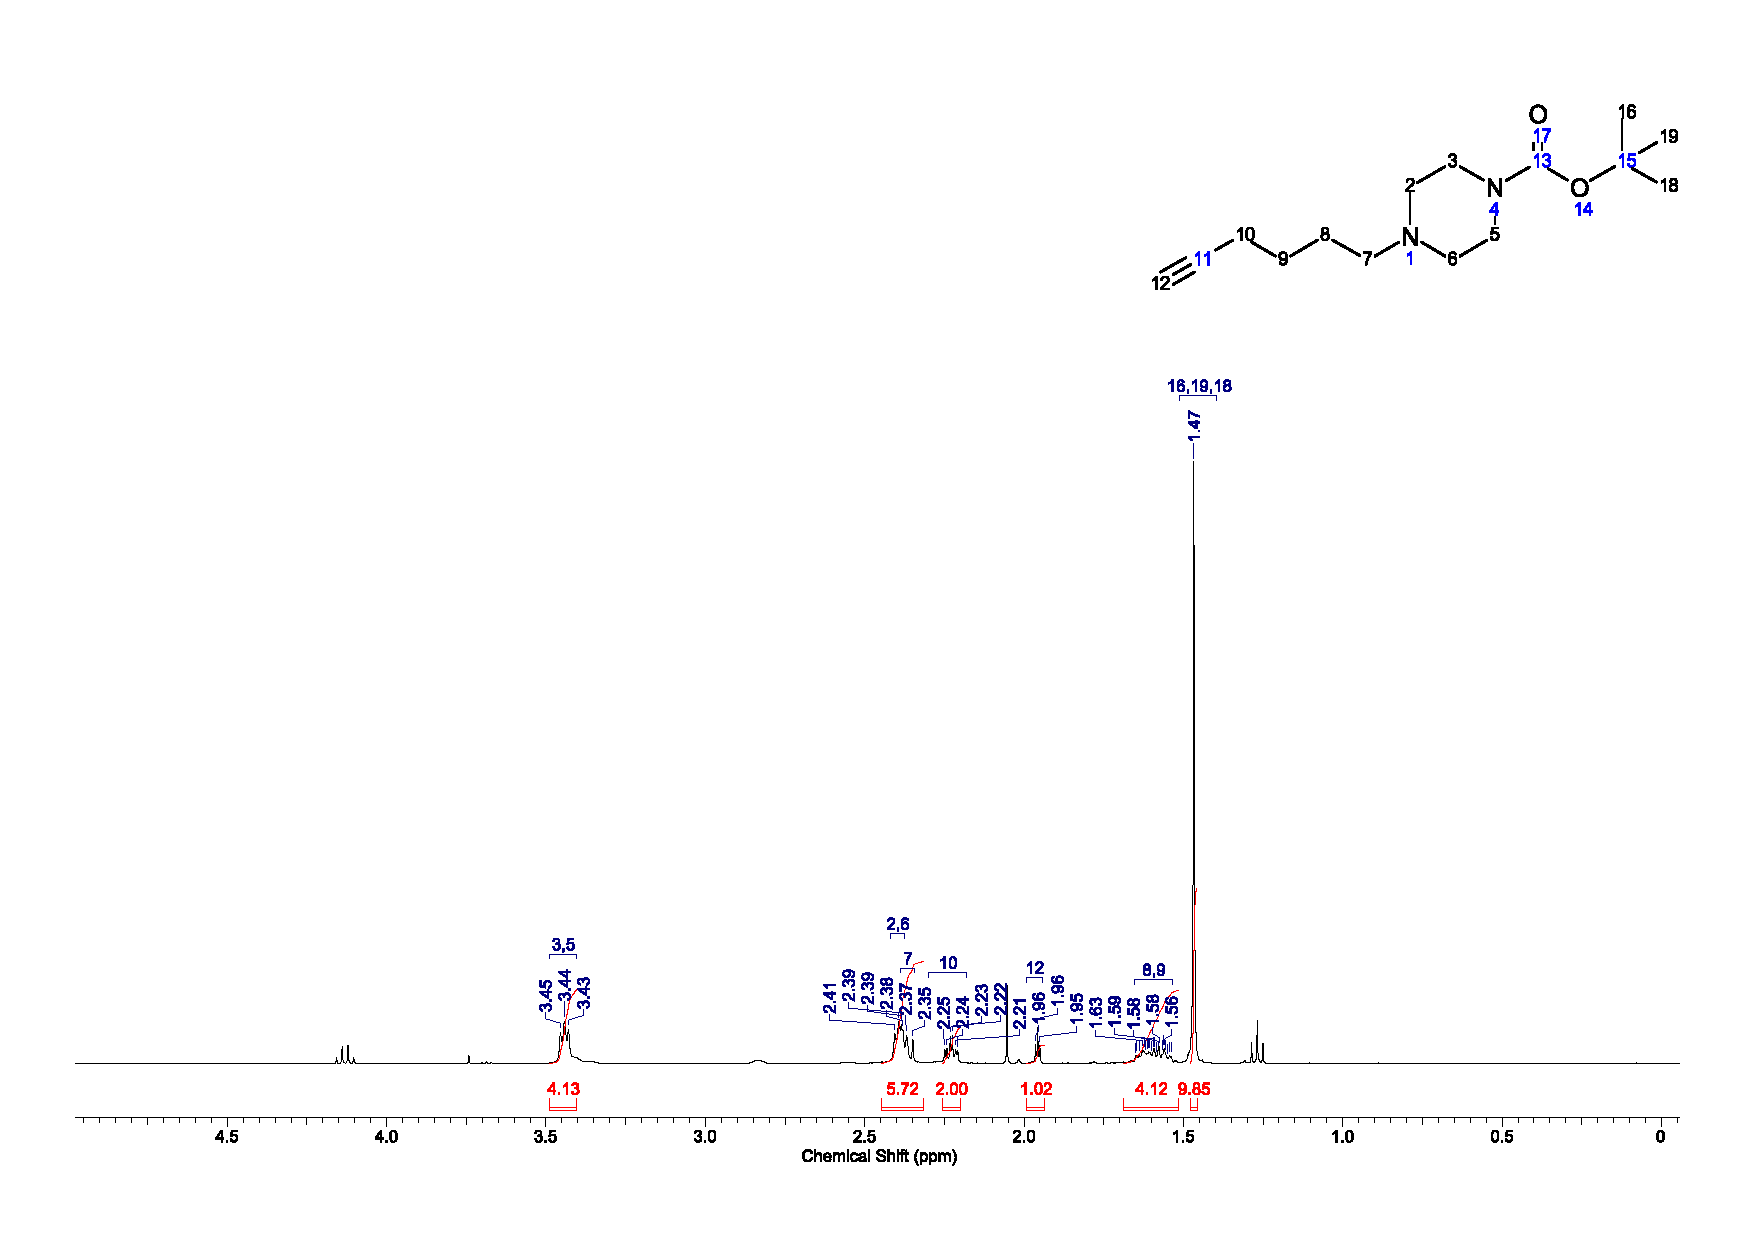
\includegraphics[ width=1.0\textwidth,height=0.43\textheight,keepaspectratio]{hexpipboc_H.pdf}
		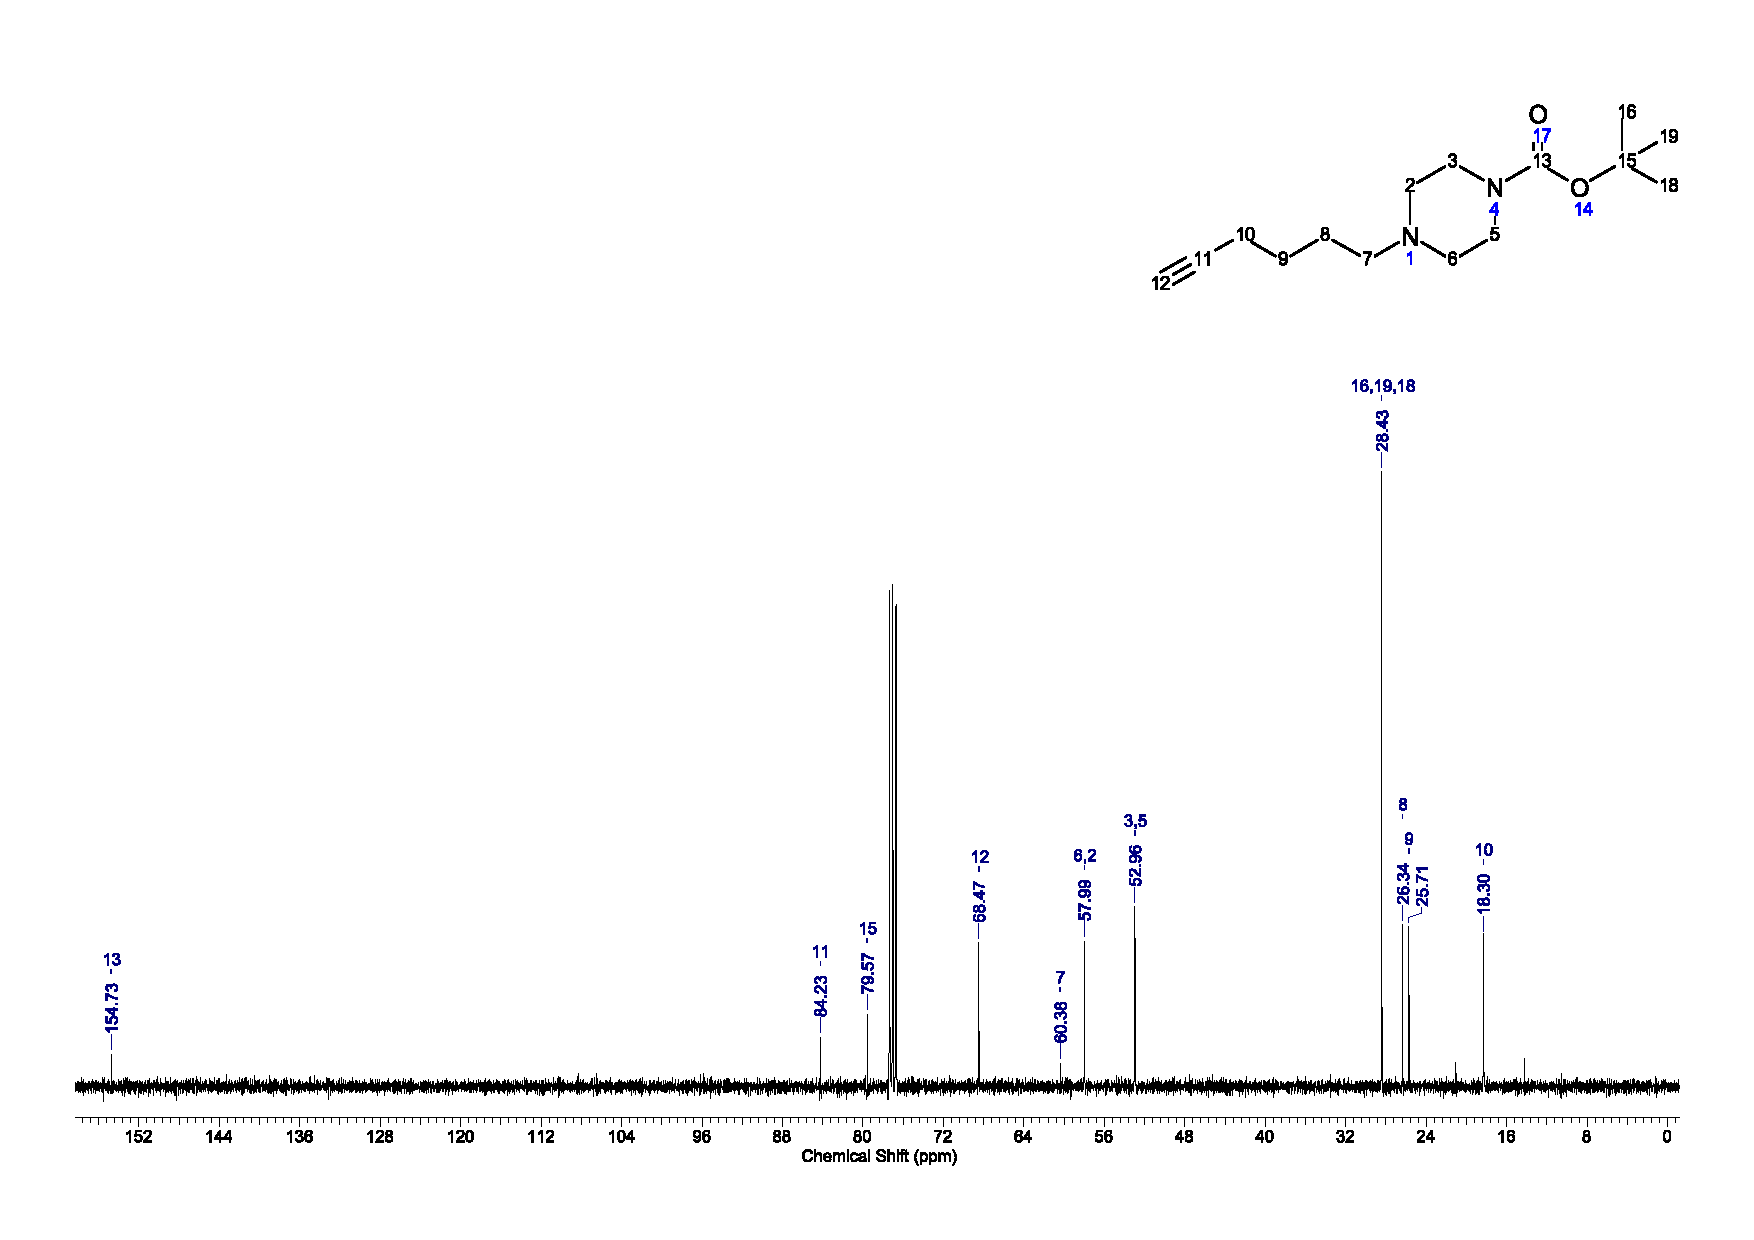
\includegraphics[ width=1.0\textwidth,height=0.43\textheight,keepaspectratio]{hexpipboc_C.pdf}
	%\caption{\compound{cmpd:hexpipboc}}
\end{figure}

\subsection{1-(Hex-5-yn-1-yl)piperazine \compound{cmpd:hexpip}}

\begin{figure}[H]
	\centering
		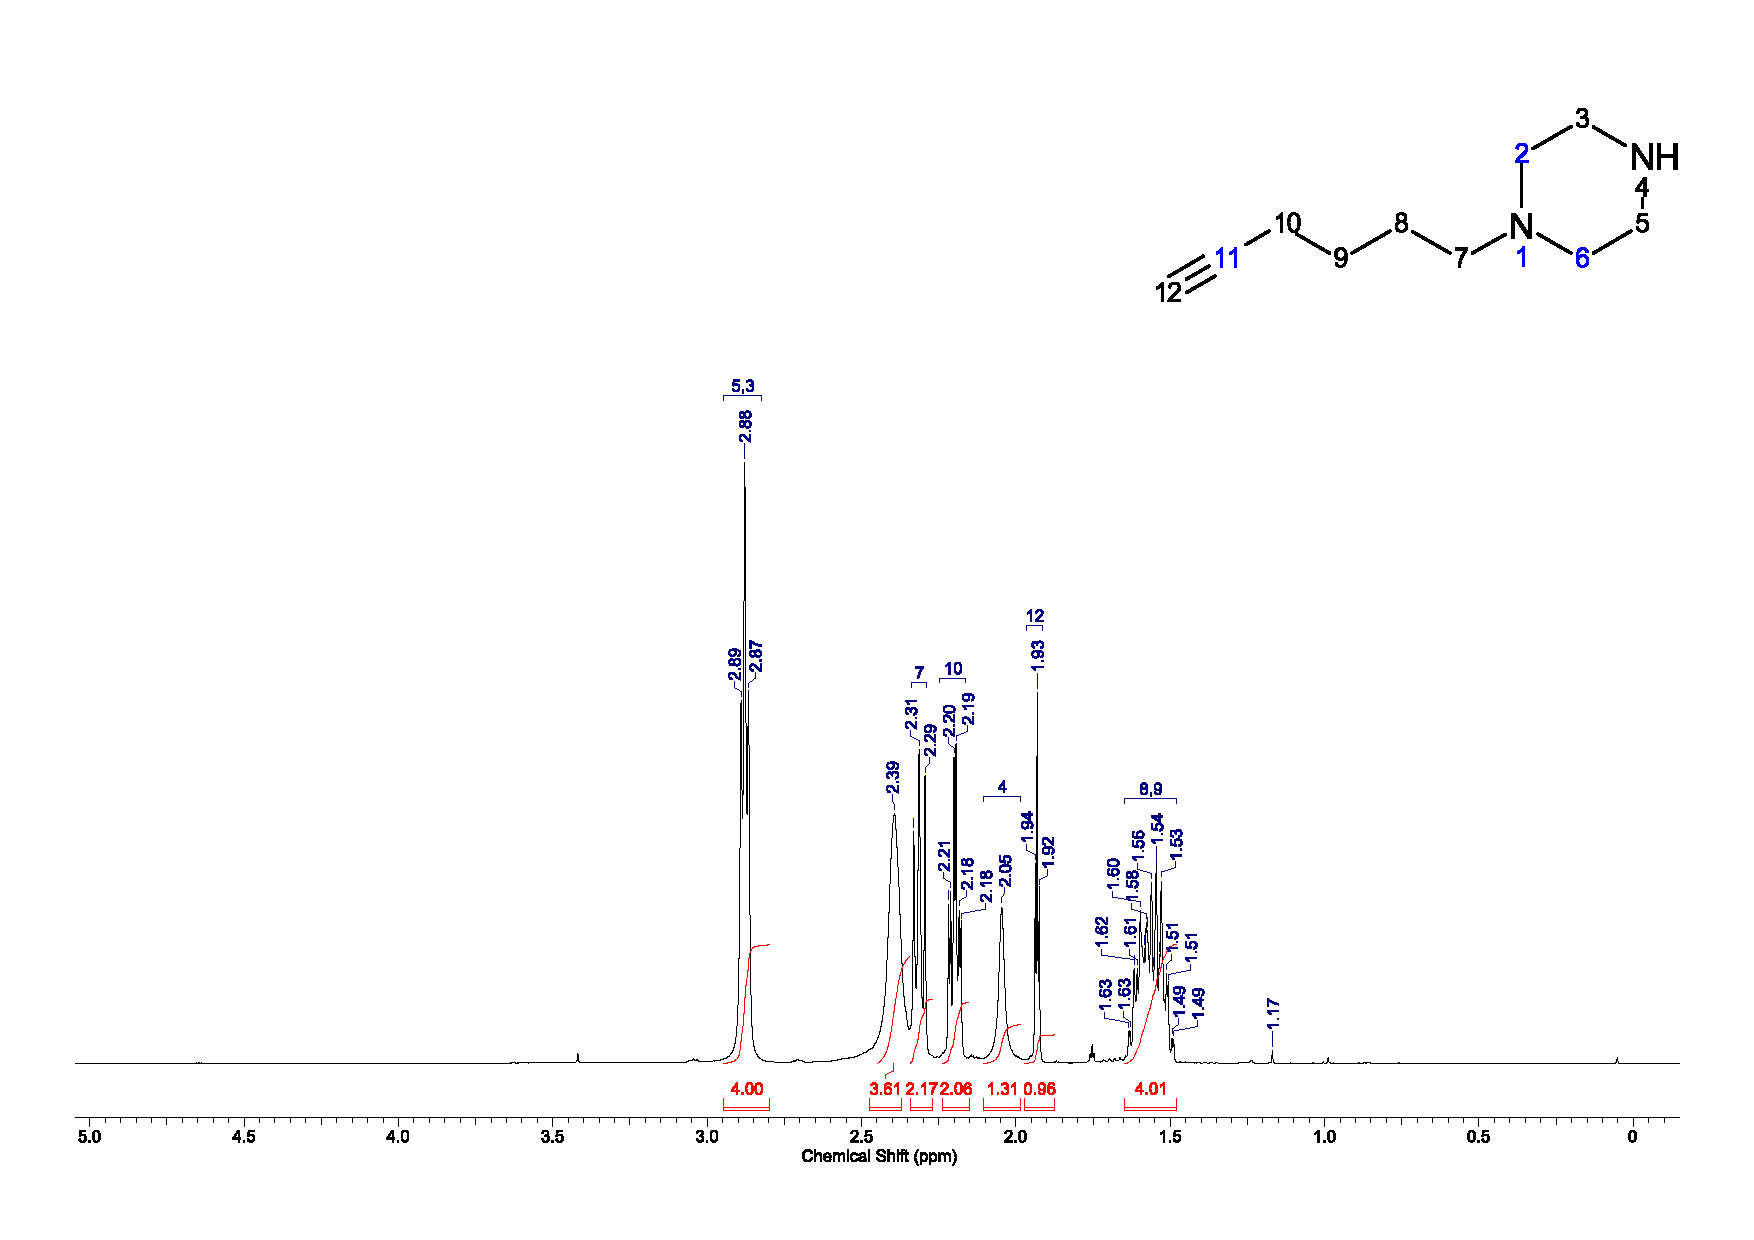
\includegraphics[ width=1.0\textwidth,height=0.43\textheight,keepaspectratio]{hexpip_H.pdf}
		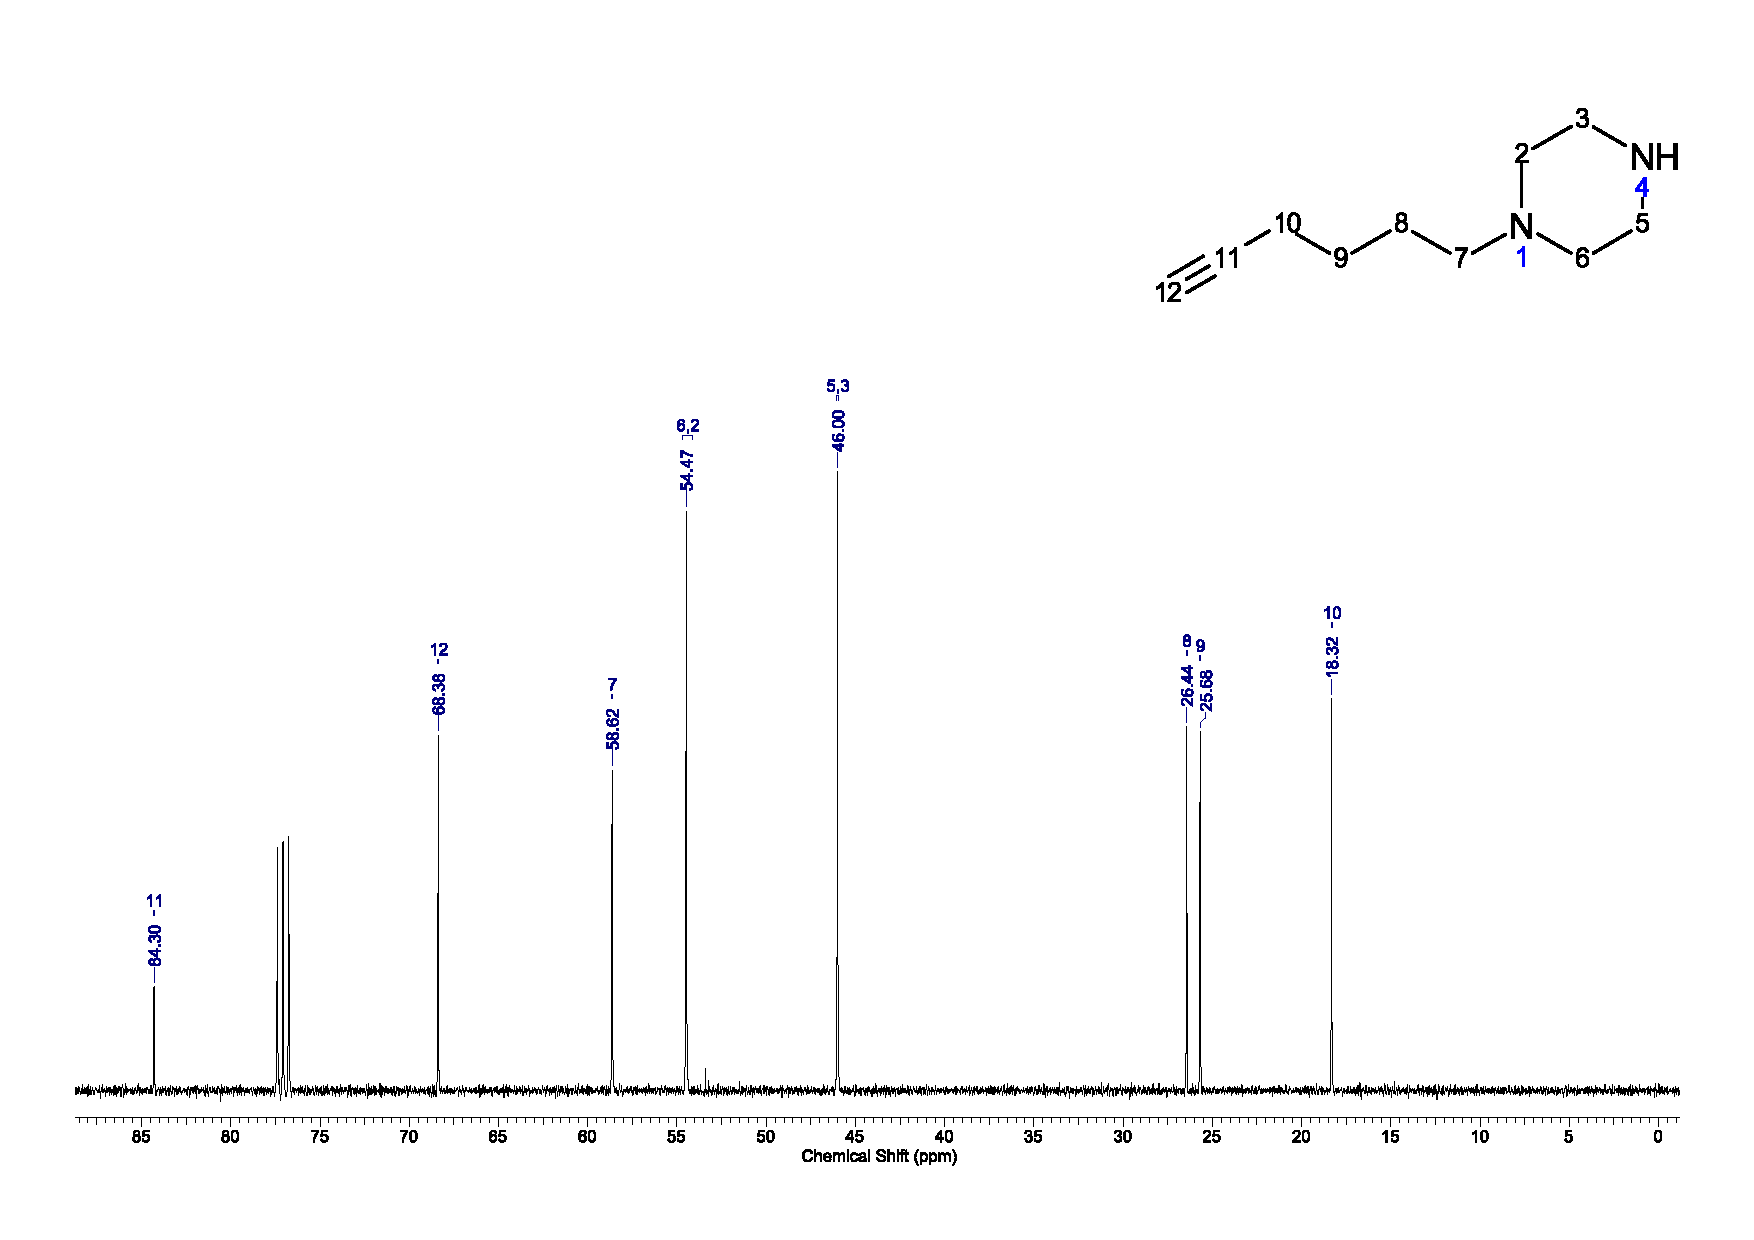
\includegraphics[ width=1.0\textwidth,height=0.43\textheight,keepaspectratio]{hexpip_C.pdf}
	%\caption{\compound{cmpd:hexpip}}
\end{figure}

\subsection{1-Cyclopropyl-6-fluoro-7-(4-(hex-5-yn-1-yl)piperazin-1-yl)-4-oxo-1,4\hyp{}dihydro\-quinoline-3-carboxylic acid \compound{cmpd:hexpipcip}}

\begin{figure}[H]
	\centering
		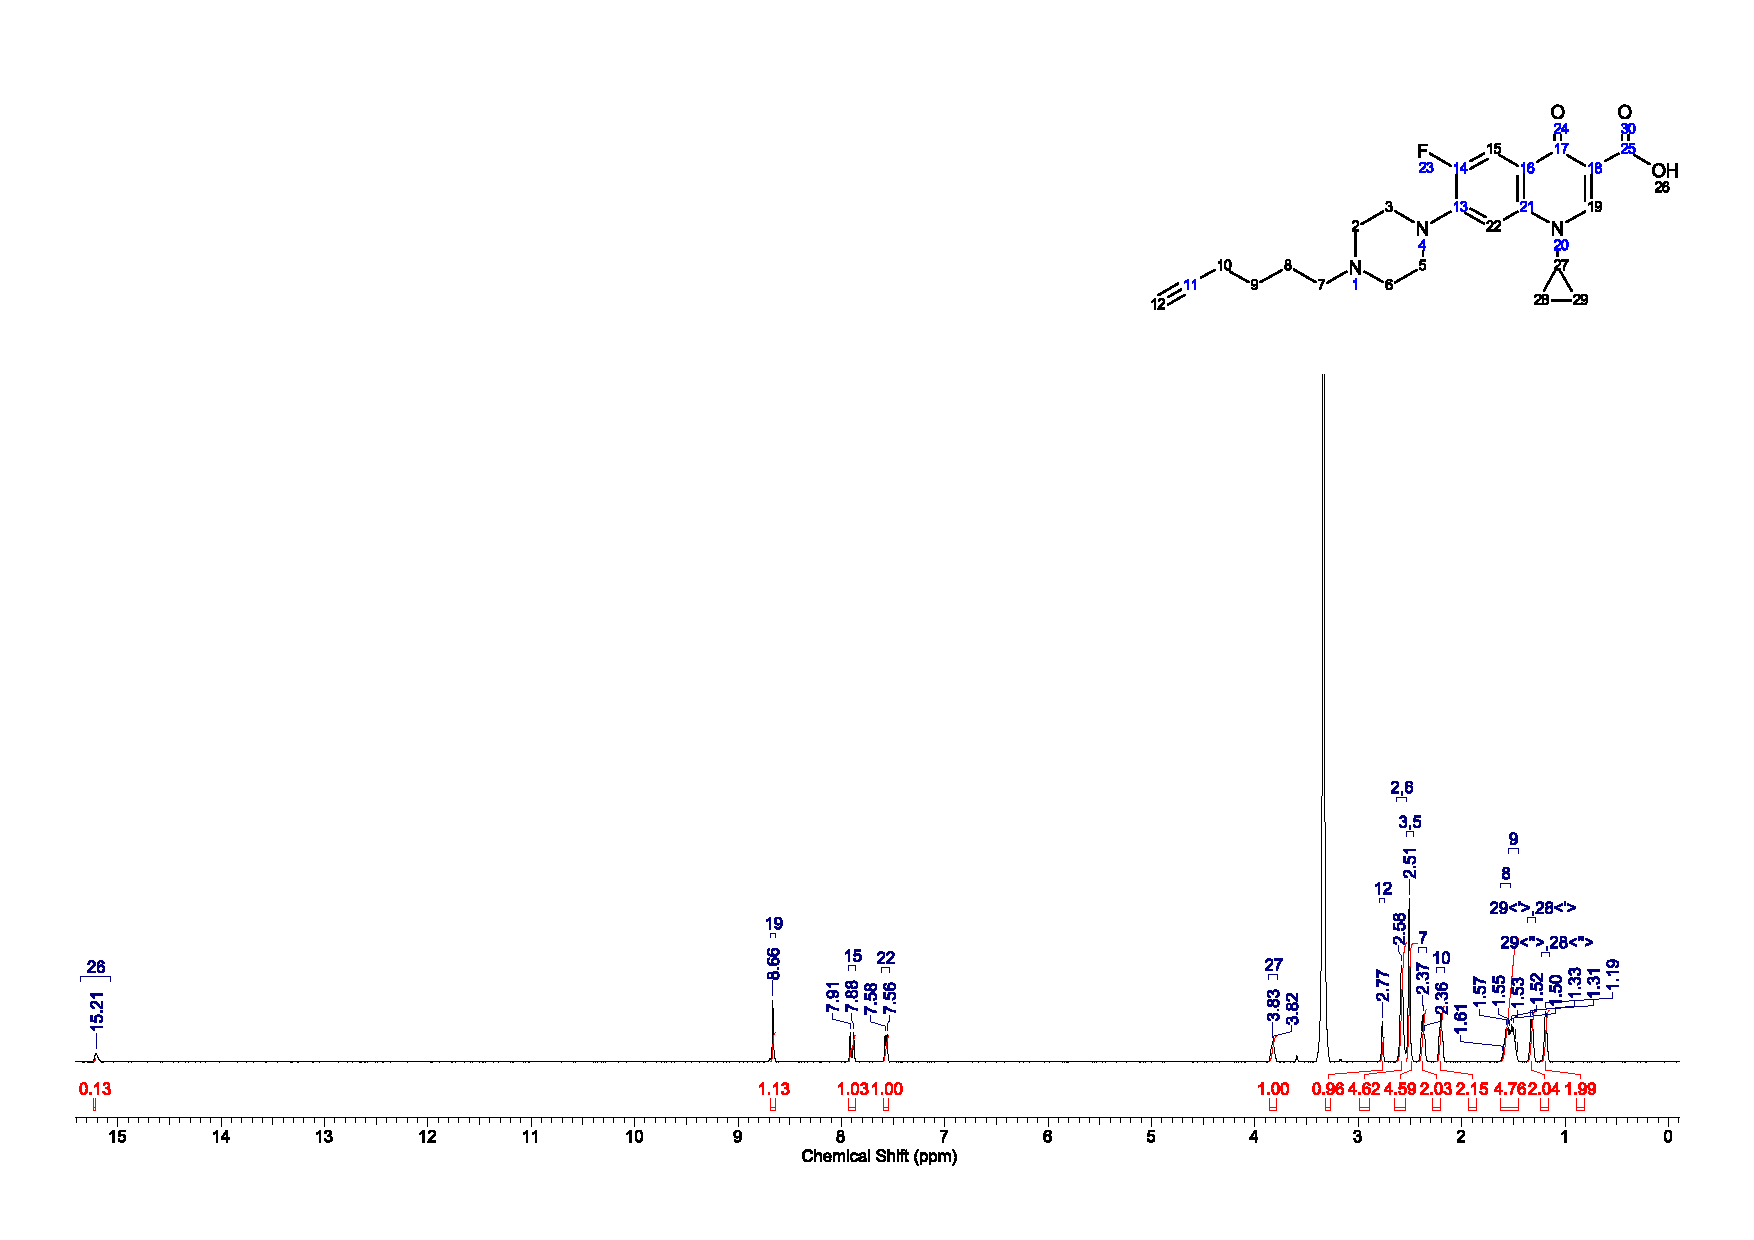
\includegraphics[ width=1.0\textwidth,height=0.43\textheight,keepaspectratio,height=0.43\textheight,keepaspectratio]{hexpipcip_H.pdf}
		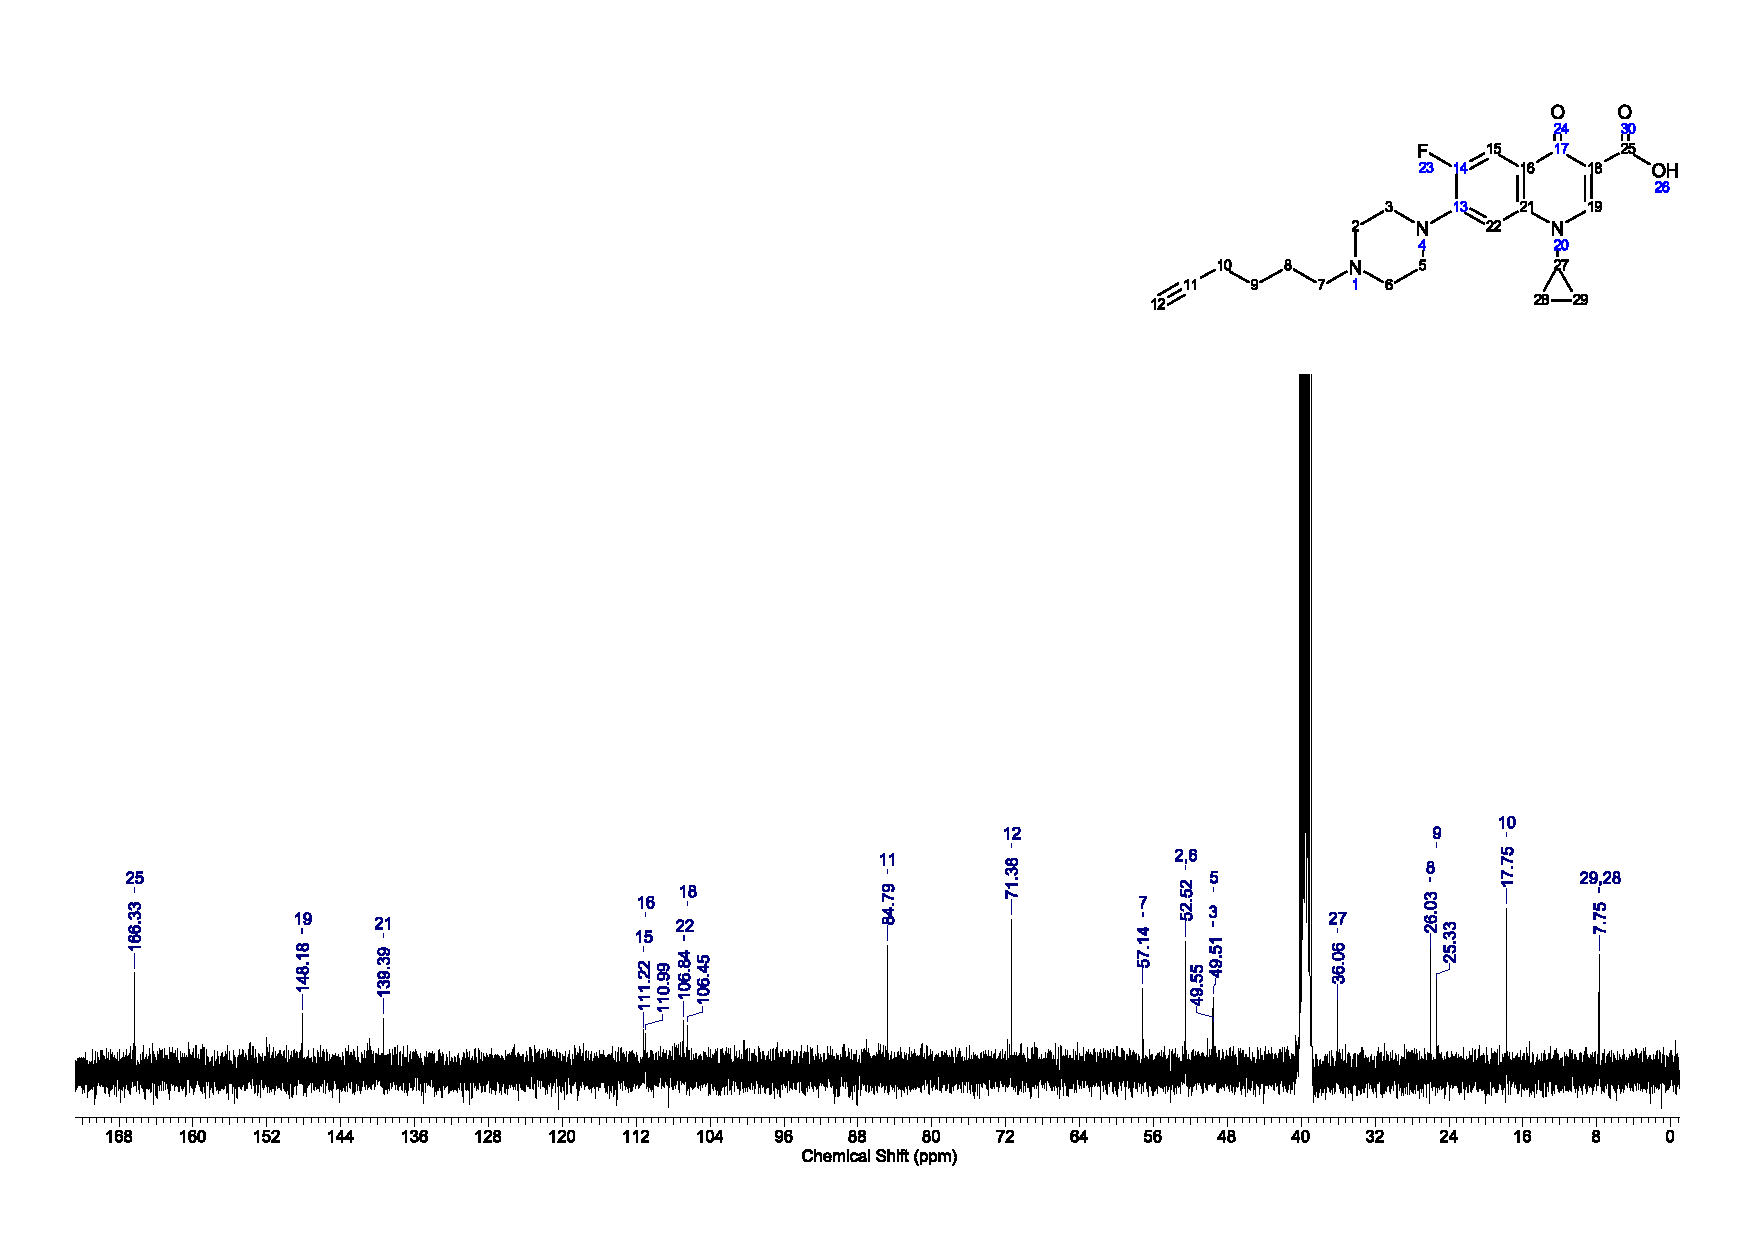
\includegraphics[ width=1.0\textwidth,height=0.43\textheight,keepaspectratio,height=0.43\textheight,keepaspectratio]{hexpipcip_C.pdf}
	%\caption{\compound{cmpd:hexpipcip}}
\end{figure}